% Options for packages loaded elsewhere
\PassOptionsToPackage{unicode}{hyperref}
\PassOptionsToPackage{hyphens}{url}
\PassOptionsToPackage{dvipsnames,svgnames,x11names}{xcolor}
%
\documentclass[
  a4paper,
  DIV=11,
  numbers=noendperiod]{scrreprt}

\usepackage{amsmath,amssymb}
\usepackage{iftex}
\ifPDFTeX
  \usepackage[T1]{fontenc}
  \usepackage[utf8]{inputenc}
  \usepackage{textcomp} % provide euro and other symbols
\else % if luatex or xetex
  \usepackage{unicode-math}
  \defaultfontfeatures{Scale=MatchLowercase}
  \defaultfontfeatures[\rmfamily]{Ligatures=TeX,Scale=1}
\fi
\usepackage{lmodern}
\ifPDFTeX\else  
    % xetex/luatex font selection
\fi
% Use upquote if available, for straight quotes in verbatim environments
\IfFileExists{upquote.sty}{\usepackage{upquote}}{}
\IfFileExists{microtype.sty}{% use microtype if available
  \usepackage[]{microtype}
  \UseMicrotypeSet[protrusion]{basicmath} % disable protrusion for tt fonts
}{}
\makeatletter
\@ifundefined{KOMAClassName}{% if non-KOMA class
  \IfFileExists{parskip.sty}{%
    \usepackage{parskip}
  }{% else
    \setlength{\parindent}{0pt}
    \setlength{\parskip}{6pt plus 2pt minus 1pt}}
}{% if KOMA class
  \KOMAoptions{parskip=half}}
\makeatother
\usepackage{xcolor}
\setlength{\emergencystretch}{3em} % prevent overfull lines
\setcounter{secnumdepth}{-\maxdimen} % remove section numbering
% Make \paragraph and \subparagraph free-standing
\ifx\paragraph\undefined\else
  \let\oldparagraph\paragraph
  \renewcommand{\paragraph}[1]{\oldparagraph{#1}\mbox{}}
\fi
\ifx\subparagraph\undefined\else
  \let\oldsubparagraph\subparagraph
  \renewcommand{\subparagraph}[1]{\oldsubparagraph{#1}\mbox{}}
\fi


\providecommand{\tightlist}{%
  \setlength{\itemsep}{0pt}\setlength{\parskip}{0pt}}\usepackage{longtable,booktabs,array}
\usepackage{calc} % for calculating minipage widths
% Correct order of tables after \paragraph or \subparagraph
\usepackage{etoolbox}
\makeatletter
\patchcmd\longtable{\par}{\if@noskipsec\mbox{}\fi\par}{}{}
\makeatother
% Allow footnotes in longtable head/foot
\IfFileExists{footnotehyper.sty}{\usepackage{footnotehyper}}{\usepackage{footnote}}
\makesavenoteenv{longtable}
\usepackage{graphicx}
\makeatletter
\def\maxwidth{\ifdim\Gin@nat@width>\linewidth\linewidth\else\Gin@nat@width\fi}
\def\maxheight{\ifdim\Gin@nat@height>\textheight\textheight\else\Gin@nat@height\fi}
\makeatother
% Scale images if necessary, so that they will not overflow the page
% margins by default, and it is still possible to overwrite the defaults
% using explicit options in \includegraphics[width, height, ...]{}
\setkeys{Gin}{width=\maxwidth,height=\maxheight,keepaspectratio}
% Set default figure placement to htbp
\makeatletter
\def\fps@figure{htbp}
\makeatother
% definitions for citeproc citations
\NewDocumentCommand\citeproctext{}{}
\NewDocumentCommand\citeproc{mm}{%
  \begingroup\def\citeproctext{#2}\cite{#1}\endgroup}
\makeatletter
 % allow citations to break across lines
 \let\@cite@ofmt\@firstofone
 % avoid brackets around text for \cite:
 \def\@biblabel#1{}
 \def\@cite#1#2{{#1\if@tempswa , #2\fi}}
\makeatother
\newlength{\cslhangindent}
\setlength{\cslhangindent}{1.5em}
\newlength{\csllabelwidth}
\setlength{\csllabelwidth}{3em}
\newenvironment{CSLReferences}[2] % #1 hanging-indent, #2 entry-spacing
 {\begin{list}{}{%
  \setlength{\itemindent}{0pt}
  \setlength{\leftmargin}{0pt}
  \setlength{\parsep}{0pt}
  % turn on hanging indent if param 1 is 1
  \ifodd #1
   \setlength{\leftmargin}{\cslhangindent}
   \setlength{\itemindent}{-1\cslhangindent}
  \fi
  % set entry spacing
  \setlength{\itemsep}{#2\baselineskip}}}
 {\end{list}}
\usepackage{calc}
\newcommand{\CSLBlock}[1]{\hfill\break\parbox[t]{\linewidth}{\strut\ignorespaces#1\strut}}
\newcommand{\CSLLeftMargin}[1]{\parbox[t]{\csllabelwidth}{\strut#1\strut}}
\newcommand{\CSLRightInline}[1]{\parbox[t]{\linewidth - \csllabelwidth}{\strut#1\strut}}
\newcommand{\CSLIndent}[1]{\hspace{\cslhangindent}#1}

\usepackage{float}
\usepackage{tabularray}
\usepackage[normalem]{ulem}
\usepackage{graphicx}
\UseTblrLibrary{booktabs}
\UseTblrLibrary{siunitx}
\NewTableCommand{\tinytableDefineColor}[3]{\definecolor{#1}{#2}{#3}}
\newcommand{\tinytableTabularrayUnderline}[1]{\underline{#1}}
\newcommand{\tinytableTabularrayStrikeout}[1]{\sout{#1}}
\KOMAoption{captions}{tableheading}
\makeatletter
\@ifpackageloaded{tcolorbox}{}{\usepackage[skins,breakable]{tcolorbox}}
\@ifpackageloaded{fontawesome5}{}{\usepackage{fontawesome5}}
\definecolor{quarto-callout-color}{HTML}{909090}
\definecolor{quarto-callout-note-color}{HTML}{0758E5}
\definecolor{quarto-callout-important-color}{HTML}{CC1914}
\definecolor{quarto-callout-warning-color}{HTML}{EB9113}
\definecolor{quarto-callout-tip-color}{HTML}{00A047}
\definecolor{quarto-callout-caution-color}{HTML}{FC5300}
\definecolor{quarto-callout-color-frame}{HTML}{acacac}
\definecolor{quarto-callout-note-color-frame}{HTML}{4582ec}
\definecolor{quarto-callout-important-color-frame}{HTML}{d9534f}
\definecolor{quarto-callout-warning-color-frame}{HTML}{f0ad4e}
\definecolor{quarto-callout-tip-color-frame}{HTML}{02b875}
\definecolor{quarto-callout-caution-color-frame}{HTML}{fd7e14}
\makeatother
\makeatletter
\@ifpackageloaded{caption}{}{\usepackage{caption}}
\AtBeginDocument{%
\ifdefined\contentsname
  \renewcommand*\contentsname{Table of contents}
\else
  \newcommand\contentsname{Table of contents}
\fi
\ifdefined\listfigurename
  \renewcommand*\listfigurename{List of Figures}
\else
  \newcommand\listfigurename{List of Figures}
\fi
\ifdefined\listtablename
  \renewcommand*\listtablename{List of Tables}
\else
  \newcommand\listtablename{List of Tables}
\fi
\ifdefined\figurename
  \renewcommand*\figurename{Figure}
\else
  \newcommand\figurename{Figure}
\fi
\ifdefined\tablename
  \renewcommand*\tablename{Table}
\else
  \newcommand\tablename{Table}
\fi
}
\@ifpackageloaded{float}{}{\usepackage{float}}
\floatstyle{ruled}
\@ifundefined{c@chapter}{\newfloat{codelisting}{h}{lop}}{\newfloat{codelisting}{h}{lop}[chapter]}
\floatname{codelisting}{Listing}
\newcommand*\listoflistings{\listof{codelisting}{List of Listings}}
\makeatother
\makeatletter
\makeatother
\makeatletter
\@ifpackageloaded{caption}{}{\usepackage{caption}}
\@ifpackageloaded{subcaption}{}{\usepackage{subcaption}}
\makeatother
\ifLuaTeX
  \usepackage{selnolig}  % disable illegal ligatures
\fi
\usepackage{bookmark}

\IfFileExists{xurl.sty}{\usepackage{xurl}}{} % add URL line breaks if available
\urlstyle{same} % disable monospaced font for URLs
\hypersetup{
  pdftitle={Services trade and the Indonesian third unbundling},
  pdfauthor={Krisna Gupta; Dhany S. Ratana},
  colorlinks=true,
  linkcolor={blue},
  filecolor={Maroon},
  citecolor={Blue},
  urlcolor={Blue},
  pdfcreator={LaTeX via pandoc}}

\title{Services trade and the Indonesian third unbundling}
\author{Krisna Gupta \and Dhany S. Ratana}
\date{July 14, 2024}

\begin{document}
\maketitle
\begin{abstract}
Awokowkoawkoawk.
\end{abstract}

\begin{tcolorbox}[enhanced jigsaw, colback=white, opacityback=0, bottomrule=.15mm, breakable, colbacktitle=quarto-callout-warning-color!10!white, colframe=quarto-callout-warning-color-frame, bottomtitle=1mm, rightrule=.15mm, coltitle=black, titlerule=0mm, arc=.35mm, toprule=.15mm, leftrule=.75mm, left=2mm, title=\textcolor{quarto-callout-warning-color}{\faExclamationTriangle}\hspace{0.5em}{Warning}, toptitle=1mm, opacitybacktitle=0.6]

This document is a work in progress. Please do not cite. Comments are
welcomed. For replication see
\href{https://github.com/imedkrisna/ERIA_services}{here}

\end{tcolorbox}

\section{Introduction}\label{introduction}

Trade in services is growing in importance all over the world, Indonesia
included. Figure~\ref{fig-1} shows Indonesia's export and import in
services taken from Indonesian Statistic Bureau compiled by the Central
Bank (Bank Indonesia, n.d.). Indonesia's services trade is growing
steadily from 2000, only to be interrupted by the COVID-19 pandemic.
Export service is dominated by tourism, while import services is
dominated by logistics. While the trend is increasing, it is evident
that Indonesia's import of services has always been dominating exports.

\begin{figure}

\centering{

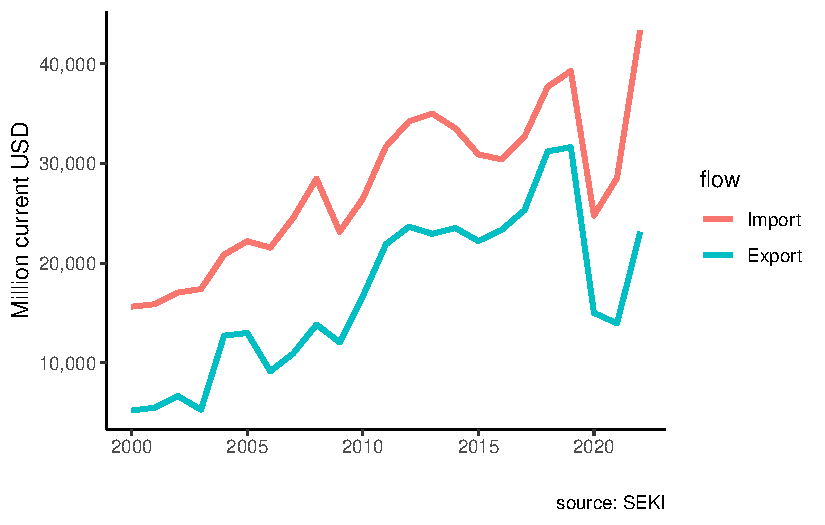
\includegraphics{services_document_files/figure-pdf/fig-1-1.pdf}

}

\caption{\label{fig-1}Indonesian trade in services}

\end{figure}%

Indonesian government often concerned with deficit trade, but trade in
services has often neglected in the discussion. Indeed, trade balance in
goods are often far outweight the deficit in its services counterpart,
as made apparent by Figure~\ref{fig-2}. However, while Indonesia's trade
balance fluctuates along with commodity prices and global demand in
general, services trade deficit is consistent. Additionally, Indonesia's
reliance on services import went up right after COVID-19 and seems to
stabilize in a higher than pre-pandemic level. With the increasing role
of services in the global trade, the deficit looks to be even more
important in Indonesia's current account in the future.

\begin{figure}

\centering{

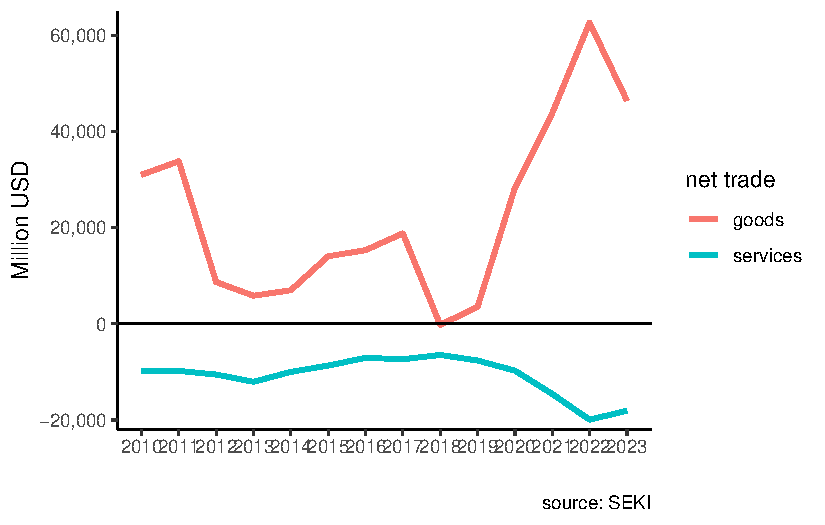
\includegraphics{services_document_files/figure-pdf/fig-2-1.pdf}

}

\caption{\label{fig-2}Net trade in goods and services of Indonesia, 200}

\end{figure}%

The importance of trade in services goes beyond current account. With
the ever decreasing cost of trade, separating a value up to tasks level
(i.e., the third unbundling) is on the horizon (Baldwin 2011; Kimura
2018). Feedback mechanism from the third unbundling may benefits
domestic manufacturing (Kimura 2018). Therefore, services trade may be
important in the next stage of globalization.

This chapter have at least two objectives. First, we explores the
general trade in services in Indonesia. We use BaTIS data (WTO/OECD
2022; Liberatore and Wettstein 2021) to show Indonesia's most important
services trade and country partners for both export and import. Trade in
services has been increasing in importance, especially in the rise of
deep trade agreements involving integration in trade in services as well
as goods (Patunru 2023). Thus, trade in services' profile of Indonesia
will be most useful to Indonesian academics and policy makers.

Secondly, we investigate the potency of the feedback mechanism from the
third unbundling a la Kimura (2018). That is, we look at how much
imported services are embedded in Indonesia's manufacturing sectors
aggregated into ICIO classifications. We do this in two ways. First, we
use ARDL (Pesaran and Smith 1995) to see whether services imports
cointegrate with manufacturing exports and GDP. Secondly, we utilize
Inter-Country Input-Output (ICIO) data from OECD (OECD 2023) to look at
the importance of services for Indonesian manufacturing.

We arrange this chapter in the following. Section 2 discusses the
development in research concerning services trade and its development in
Indonesia, section 3 discusses about data and methods, section 4
explores Indonesian services trade as well as some third unbundling
results, and section 5 concludes.

\section{Review on services trade}\label{review-on-services-trade}

kimura

gupta

\section{Data and Method}\label{data-and-method}

There are two main dataset used in this chapter. Namely, Balanced Trade
in Services (BaTIS) and the OECD Inter-Country Input-Output (ICIO)
dataset.

The BaTIS database was first launched in 2017 by World Trade
organization (WTO) and Organization of Economic Cooperation and
Development (OECD) in tandem (Liberatore and Wettstein 2021). Unlike
trade in goods, trade in services are harder to track than trade in
goods amid gap in data collection by various countries. BaTIS collect
both ways from pairs of trading partners, reconcile difference between
reporting countries' trade. BaTIS is also used to build Trade in Value
Added (TiVA) database and the ICIO database. BaTIS follows EBOPS 2010
sector classification (Liberatore et al. 2021) which can be observed in
Table~\ref{tbl-1}.

\begin{longtable}[]{@{}ll@{}}
\caption{Services classification in BaTIS}\label{tbl-1}\tabularnewline
\toprule\noalign{}
Code & Category description \\
\midrule\noalign{}
\endfirsthead
\toprule\noalign{}
Code & Category description \\
\midrule\noalign{}
\endhead
\bottomrule\noalign{}
\endlastfoot
SA & Manufacturing services on physical inputs owned by others \\
SB & Maintenance and repair services n.i.e. \\
SC & Transport \\
SD & Travel \\
SE & Construction \\
SF & Insurance and pension services \\
SG & Financial services \\
SH & Charges for the use of intellectual property n.i.e. \\
SI & Telecommunications, computer, and information services \\
SJ & Other business services \\
SK & Personal, cultural and recreational services \\
SL & Government goods and services n.i.e. \\
\end{longtable}

Trade services statistics are challenging in nature (Liberatore and
Wettstein 2021). Only around 65\% of total number of trade in services
are recorded bilaterally. Unlike trade in goods, exports are recoreded
better than imports, mainly due to advance countries being the majority
of service exporters. Only 59\% of trade value in BaTIS are fully
reported, which are the reported 65\% pair. The remaining 41\% are
estimated using share interpolations and gravity estimations. Since
BaTIS is used for other databases including TiVA and ICIO, we should
expect similar problems in these two databases.

Additionally, we also use the Indonesian trade in services statistics
compiled by the Indonesian central bank called \emph{Statistik Ekonomi
dan Keuangan Indonesia} (SEKI) (Bank Indonesia, n.d.). It records
Indonesia's trade in services in the same manner as BaTIS, but with less
detail on the trading partners. Moreover, SEKI is also used to observe
Indonesia's manufacturing GDP and goods exports and imports to estimate
the third unbundling effect.

The OECD Inter-Country Input-Output (ICIO) decribes the sale and
purchase relationships between sectors, consumers and the government
within and across borders. ICIO estimates trades amonng 76 countries and
45 unique industries based on ISIC Revision 4(OECD, 2023). The database
shows how much sectoral value added, both foreign and domestic, that is
used by a certain industry.

In this study, we focus the manufacturing sector, specifically ISIC
10-27 in the ISIC rev. 4 classification. The ICIO aggregates these
sectors into 16 sectors. We then aggregates all services that sell to
these sectors into two categories, namely domestic services and foreign
services.

On the third unbundling discussion, a good quality of firm-level data
with information of its services sourced. Unfortunately, this
information is not widely distributed in the Indonesian context. The
second-best approach is to use international input-output table, which
in this case ICIO is used.

Assume a manufacturing output and value added as a function of its
factor or production. The nest of factor of production produces fully
complementarily with its goods and services inputs. Let services inputs
be complementarily used with goods inputs, but within the value produced
by services, there is a degree of substitutability between foreign and
domestic input as such:

\begin{equation}\phantomsection\label{eq-1}{
Y_{it}=f(AS^D_{it},AS^F_{it})
}\end{equation}

for all \(i=\) manufacturing sectors and \(t=year\). A is the nest
multiplier, \(S^D_i\) and \(S^F_i\) are total services purchased by
industry \(i\), domestically and imported respectively.

Assuming a cobb-douglass relationship, then we can log-linearize
Equation~\ref{eq-1} to a simple linear system as such:

\begin{equation}\phantomsection\label{eq-2}{
y_{it}=a+\beta_d s^D_{it}+\beta_f s^F_{it}+\varepsilon_{it}
}\end{equation}

with a lower case represents the natural log of its uppercase
counterpart.

To construct the dataset for the regression, we aggregate non-factor
inputs from each manufacuring sectors, separated by whether it is from
Indonesia or from other countries. All inputs from foreign countries are
aggregated into foreign.

For comparison purpose, we also do the same for 4 countries in the
region, namely Singapore, Malaysia, Thailand and Vietnam. Data from
these 5 countries are then concatenated to add one more dimension,
countries.

\begin{table}

\caption{\label{tbl-icio}Summary Statistics from ICIO, million USD,
2002-2021.}

\centering{

\centering
\begin{tblr}[         %% tabularray outer open
]                     %% tabularray outer close
{                     %% tabularray inner open
colspec={Q[]Q[]Q[]Q[]Q[]Q[]Q[]Q[]Q[]Q[]Q[]Q[]Q[]Q[]Q[]Q[]},
cell{1}{2}={c=3,}{halign=c,},
cell{1}{5}={c=3,}{halign=c,},
cell{1}{8}={c=3,}{halign=c,},
cell{1}{11}={c=3,}{halign=c,},
cell{1}{14}={c=3,}{halign=c,},
column{1}={halign=l,},
column{2}={halign=r,},
column{3}={halign=r,},
column{4}={halign=r,},
column{5}={halign=r,},
column{6}={halign=r,},
column{7}={halign=r,},
column{8}={halign=r,},
column{9}={halign=r,},
column{10}={halign=r,},
column{11}={halign=r,},
column{12}={halign=r,},
column{13}={halign=r,},
column{14}={halign=r,},
column{15}={halign=r,},
column{16}={halign=r,},
row{1}={halign=c,},
}                     %% tabularray inner close
\toprule
& IDN &  &  & MYS &  &  & SGP &  &  & THA &  &  & VNM &  &  \\ \cmidrule[lr]{2-4}\cmidrule[lr]{5-7}\cmidrule[lr]{8-10}\cmidrule[lr]{11-13}\cmidrule[lr]{14-16}
& Mean & Median & SD & Mean & Median & SD & Mean & Median & SD & Mean & Median & SD & Mean & Median & SD \\ \midrule %% TinyTableHeader
value added         & \num{8150.56}  & \num{4815.90}  & \num{12191.95} & \num{2766.19}  & \num{1732.80} & \num{3319.24}  & \num{2836.22}  & \num{815.10}  & \num{4872.95}  & \num{4748.31}  & \num{3105.10}  & \num{4455.62}  & \num{2407.22}  & \num{1334.80} & \num{2923.18}  \\
output              & \num{21529.33} & \num{14574.60} & \num{29317.48} & \num{14400.86} & \num{7912.95} & \num{17714.54} & \num{10661.39} & \num{3276.50} & \num{18717.97} & \num{21049.73} & \num{13258.20} & \num{21692.46} & \num{12012.06} & \num{6232.75} & \num{16496.08} \\
domestic services   & \num{3735.21}  & \num{2860.40}  & \num{4176.07}  & \num{2279.68}  & \num{1285.15} & \num{2822.41}  & \num{2605.90}  & \num{810.15}  & \num{4881.07}  & \num{4128.23}  & \num{2222.00}  & \num{4253.37}  & \num{1272.77}  & \num{593.30}  & \num{1798.97}  \\
foreign services    & \num{420.05}   & \num{338.55}   & \num{339.95}   & \num{799.45}   & \num{438.50}  & \num{1192.44}  & \num{1392.83}  & \num{326.00}  & \num{3350.58}  & \num{1130.36}  & \num{758.10}   & \num{1068.89}  & \num{486.01}   & \num{277.25}  & \num{638.18}   \\
domestic goods      & \num{7123.05}  & \num{4349.30}  & \num{12296.21} & \num{5301.85}  & \num{2876.10} & \num{7371.51}  & \num{2207.18}  & \num{556.05}  & \num{4399.66}  & \num{6569.26}  & \num{2647.85}  & \num{8642.28}  & \num{4864.10}  & \num{1793.65} & \num{9620.71}  \\
foreign goods       & \num{10240.63} & \num{7311.50}  & \num{12983.59} & \num{6009.49}  & \num{3587.05} & \num{8289.09}  & \num{4445.96}  & \num{1385.45} & \num{7009.54}  & \num{9211.32}  & \num{6926.45}  & \num{8347.44}  & \num{5379.88}  & \num{3120.60} & \num{6332.25}  \\
for. services share & \num{2.45}     & \num{2.31}     & \num{1.34}     & \num{5.61}     & \num{5.43}    & \num{1.73}     & \num{10.50}    & \num{9.52}    & \num{5.07}     & \num{5.72}     & \num{5.66}     & \num{1.25}     & \num{4.53}     & \num{4.36}    & \num{1.18}     \\
dom. services share & \num{18.55}    & \num{17.77}    & \num{5.41}     & \num{15.79}    & \num{15.93}   & \num{3.59}     & \num{25.57}    & \num{25.91}   & \num{6.74}     & \num{19.54}    & \num{19.54}    & \num{3.28}     & \num{10.67}    & \num{10.20}   & \num{3.13}     \\
for. goods share    & \num{50.30}    & \num{50.87}    & \num{11.98}    & \num{44.01}    & \num{44.64}   & \num{12.13}    & \num{45.22}    & \num{45.79}   & \num{10.05}    & \num{47.85}    & \num{45.81}    & \num{9.05}     & \num{50.71}    & \num{52.91}   & \num{11.90}    \\
dom. goods share    & \num{28.60}    & \num{29.03}    & \num{8.57}     & \num{34.41}    & \num{34.15}   & \num{10.77}    & \num{18.20}    & \num{16.66}   & \num{7.75}     & \num{26.77}    & \num{27.57}    & \num{7.73}     & \num{33.86}    & \num{32.36}   & \num{11.66}    \\
\bottomrule
\end{tblr}

}

\end{table}%

Lastly, we run 6 fixed effect panel regressions. The first panel
consists of two indices, country and sector, which both dummies are used
as a fixed effect. The other 5 panels are fixed effect regressions by
country, where only sectoral fixed effect is used. This way, we can
discuss difference in coefficient between selected countries in the
region. We use output and value added as our \(y_i\), so we will have 12
fixed effect panel regressions in total.

The main variable of interest is \(\beta_f\). The third unbundling
suggests that since firms can now unbundle tasks up to service level,
firms who can unbundle its services tasks will theoretically perform
better, shown in its value added and output. Likewise, industries with
easier services unbundling will benefited more from services trade since
there will be more firms able to exploit the third unbundling in these
industries. Therefore, we expect to see a \(\beta_f>0\).

Given the limitation of ICIO and its underlying sources (i.e., BaTIS),
macro level analysis is added to complement the analysis. We use SEKI,
Indonesian database compiled by Bank Indonesia, the central bank, to get
services trade, manufactures trade, and manufacturing output. We perform
ARDL analysis (Pesaran and Smith 1995) to see whether services trade
cointegrates with manufacturing output and export.

We run four specifications:

\begin{equation}\phantomsection\label{eq-3}{
\begin{equation}
\begin{align}
exM_t&=\alpha_0+\alpha_1 exM_{t-1}+\alpha_2 imM_t+\alpha_3 imSev_t+\nu_i \\
exM_t&=\gamma_0+\gamma_1 exM_{t-1}+\gamma_2 imM_t+\gamma_3 imSev_t+ \\ \gamma_4 imM_{t-1}+\gamma_5 imSev_{t-1}+\upsilon_i \\
pdb_t&=\delta_0+\delta_1 exM_{t-1}+\delta_2 imM_t+\delta_3 imSev_t+\omega_i \\
pdb_t&=\theta_0+\theta_1 exM_{t-1}+\theta_2 imM_t+\theta_3 imSev_t+ \\ \theta_4 imM_{t-1}+\theta_5 imSev_{t-1}+\eta_i
\end{align}
\end{equation}
}\end{equation}

where \(exM\) is log manufacturing exports, \(pdb\) is log manufacturing
GDP, \(imM\) is log manufacturing imports and \(imSev\) is log services
imports, all for Indonesian level in time \(t\), where \(t\) is from
2005 to 2023. The data availability is restricted by the services import
which starts from 2005 in the SEKI data. Specifications that we run are
\texttt{ARDL(1,0,0)}, the least restrictive, and \texttt{ARDL(1,1,1)}
which is considered from AIC, BIC and RMSE (Pesaran and Smith 1995;
Natsiopoulos and Tzeremes 2022).

\section{Discussions}\label{discussions}

\subsection{Indonesian trade in
services}\label{indonesian-trade-in-services}

Figure~\ref{fig-S} shows total trade in services in 2021 in million
current USD taken from BaTIS. Categories are based on the
Table~\ref{tbl-1}. Figure~\ref{fig-CX} and Figure~\ref{fig-CM} shows
Indonesia's top 6 exporter and importer of services in 2021. Singapore
is the most important partner in trade in services for Indonesia. China,
on the other hand, is the main buyer of Indonesia's services export.
Looking at Figure~\ref{fig-SX} and Figure~\ref{fig-SM}, It is evident
that Indonesia's imports dominates exports in all categories bar travel
(SD). Additionally, the highest traded services in Indonesia are
transport (SC) and business services (SJ), aligned with global trade
statistics (Liberatore et al. 2021).

\begin{figure}

\begin{minipage}{0.50\linewidth}

\centering{

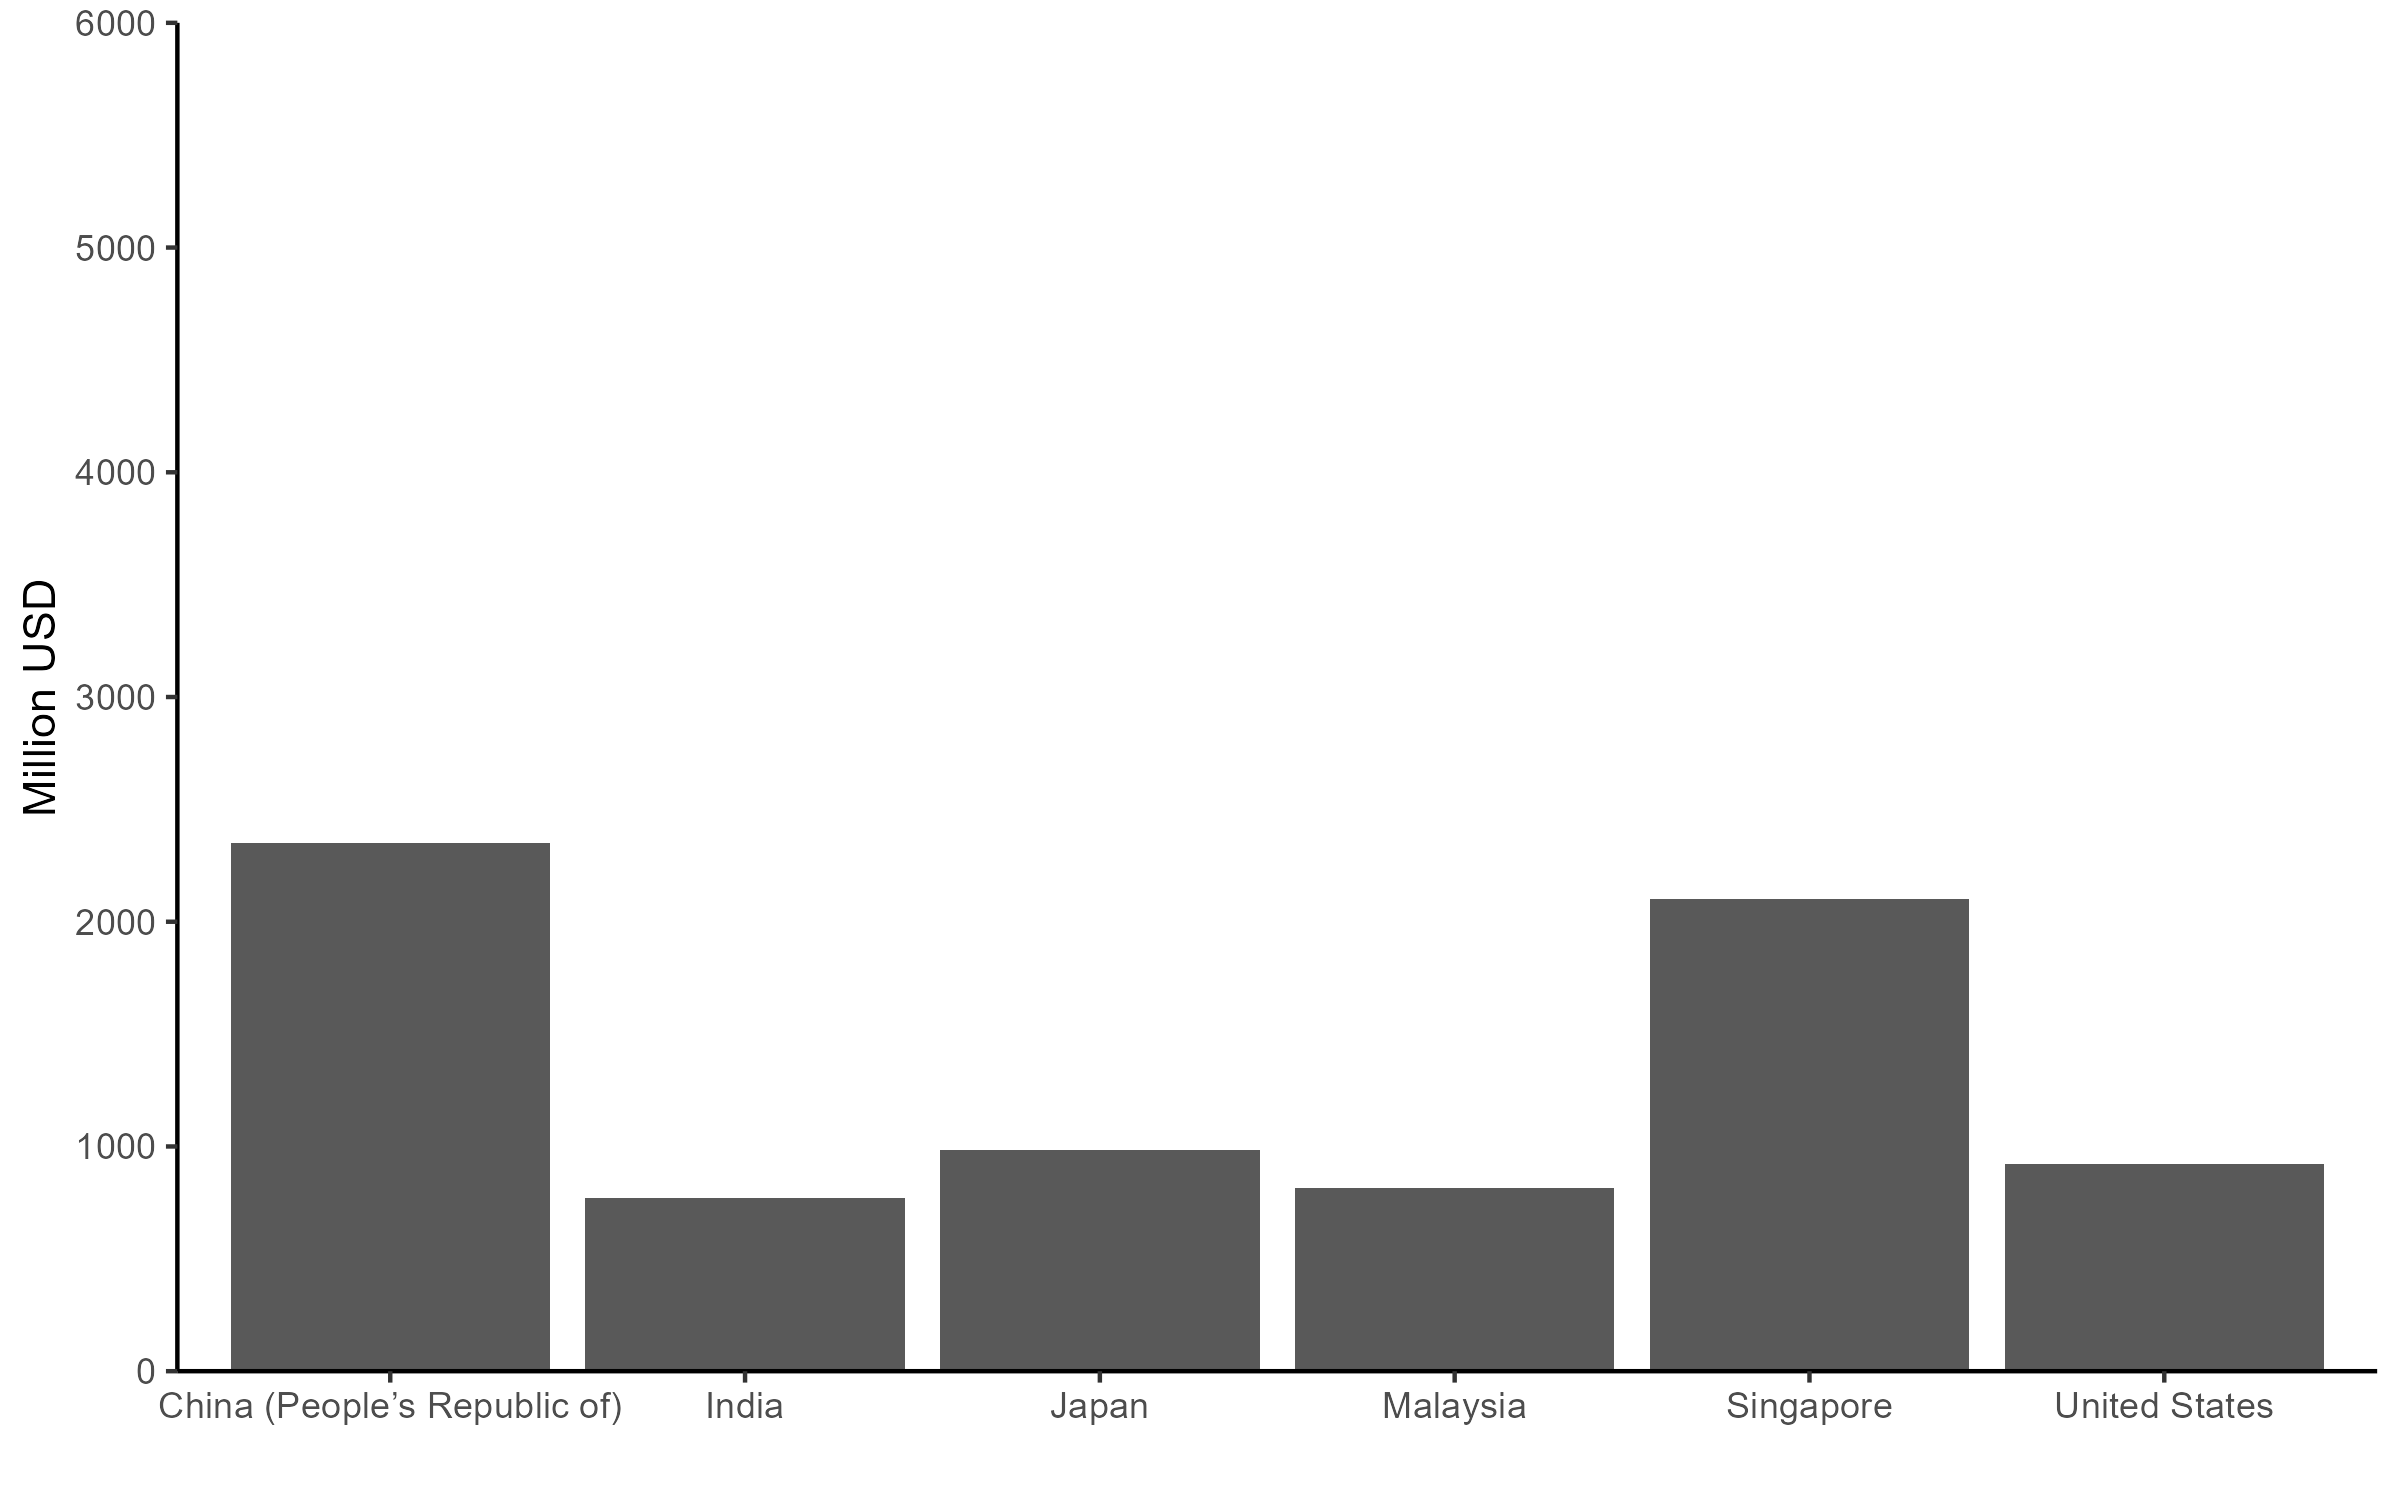
\includegraphics{plot/allcx.png}

}

\subcaption{\label{fig-CX}Indonesia's exports by partner, 2021}

\end{minipage}%
%
\begin{minipage}{0.50\linewidth}

\centering{

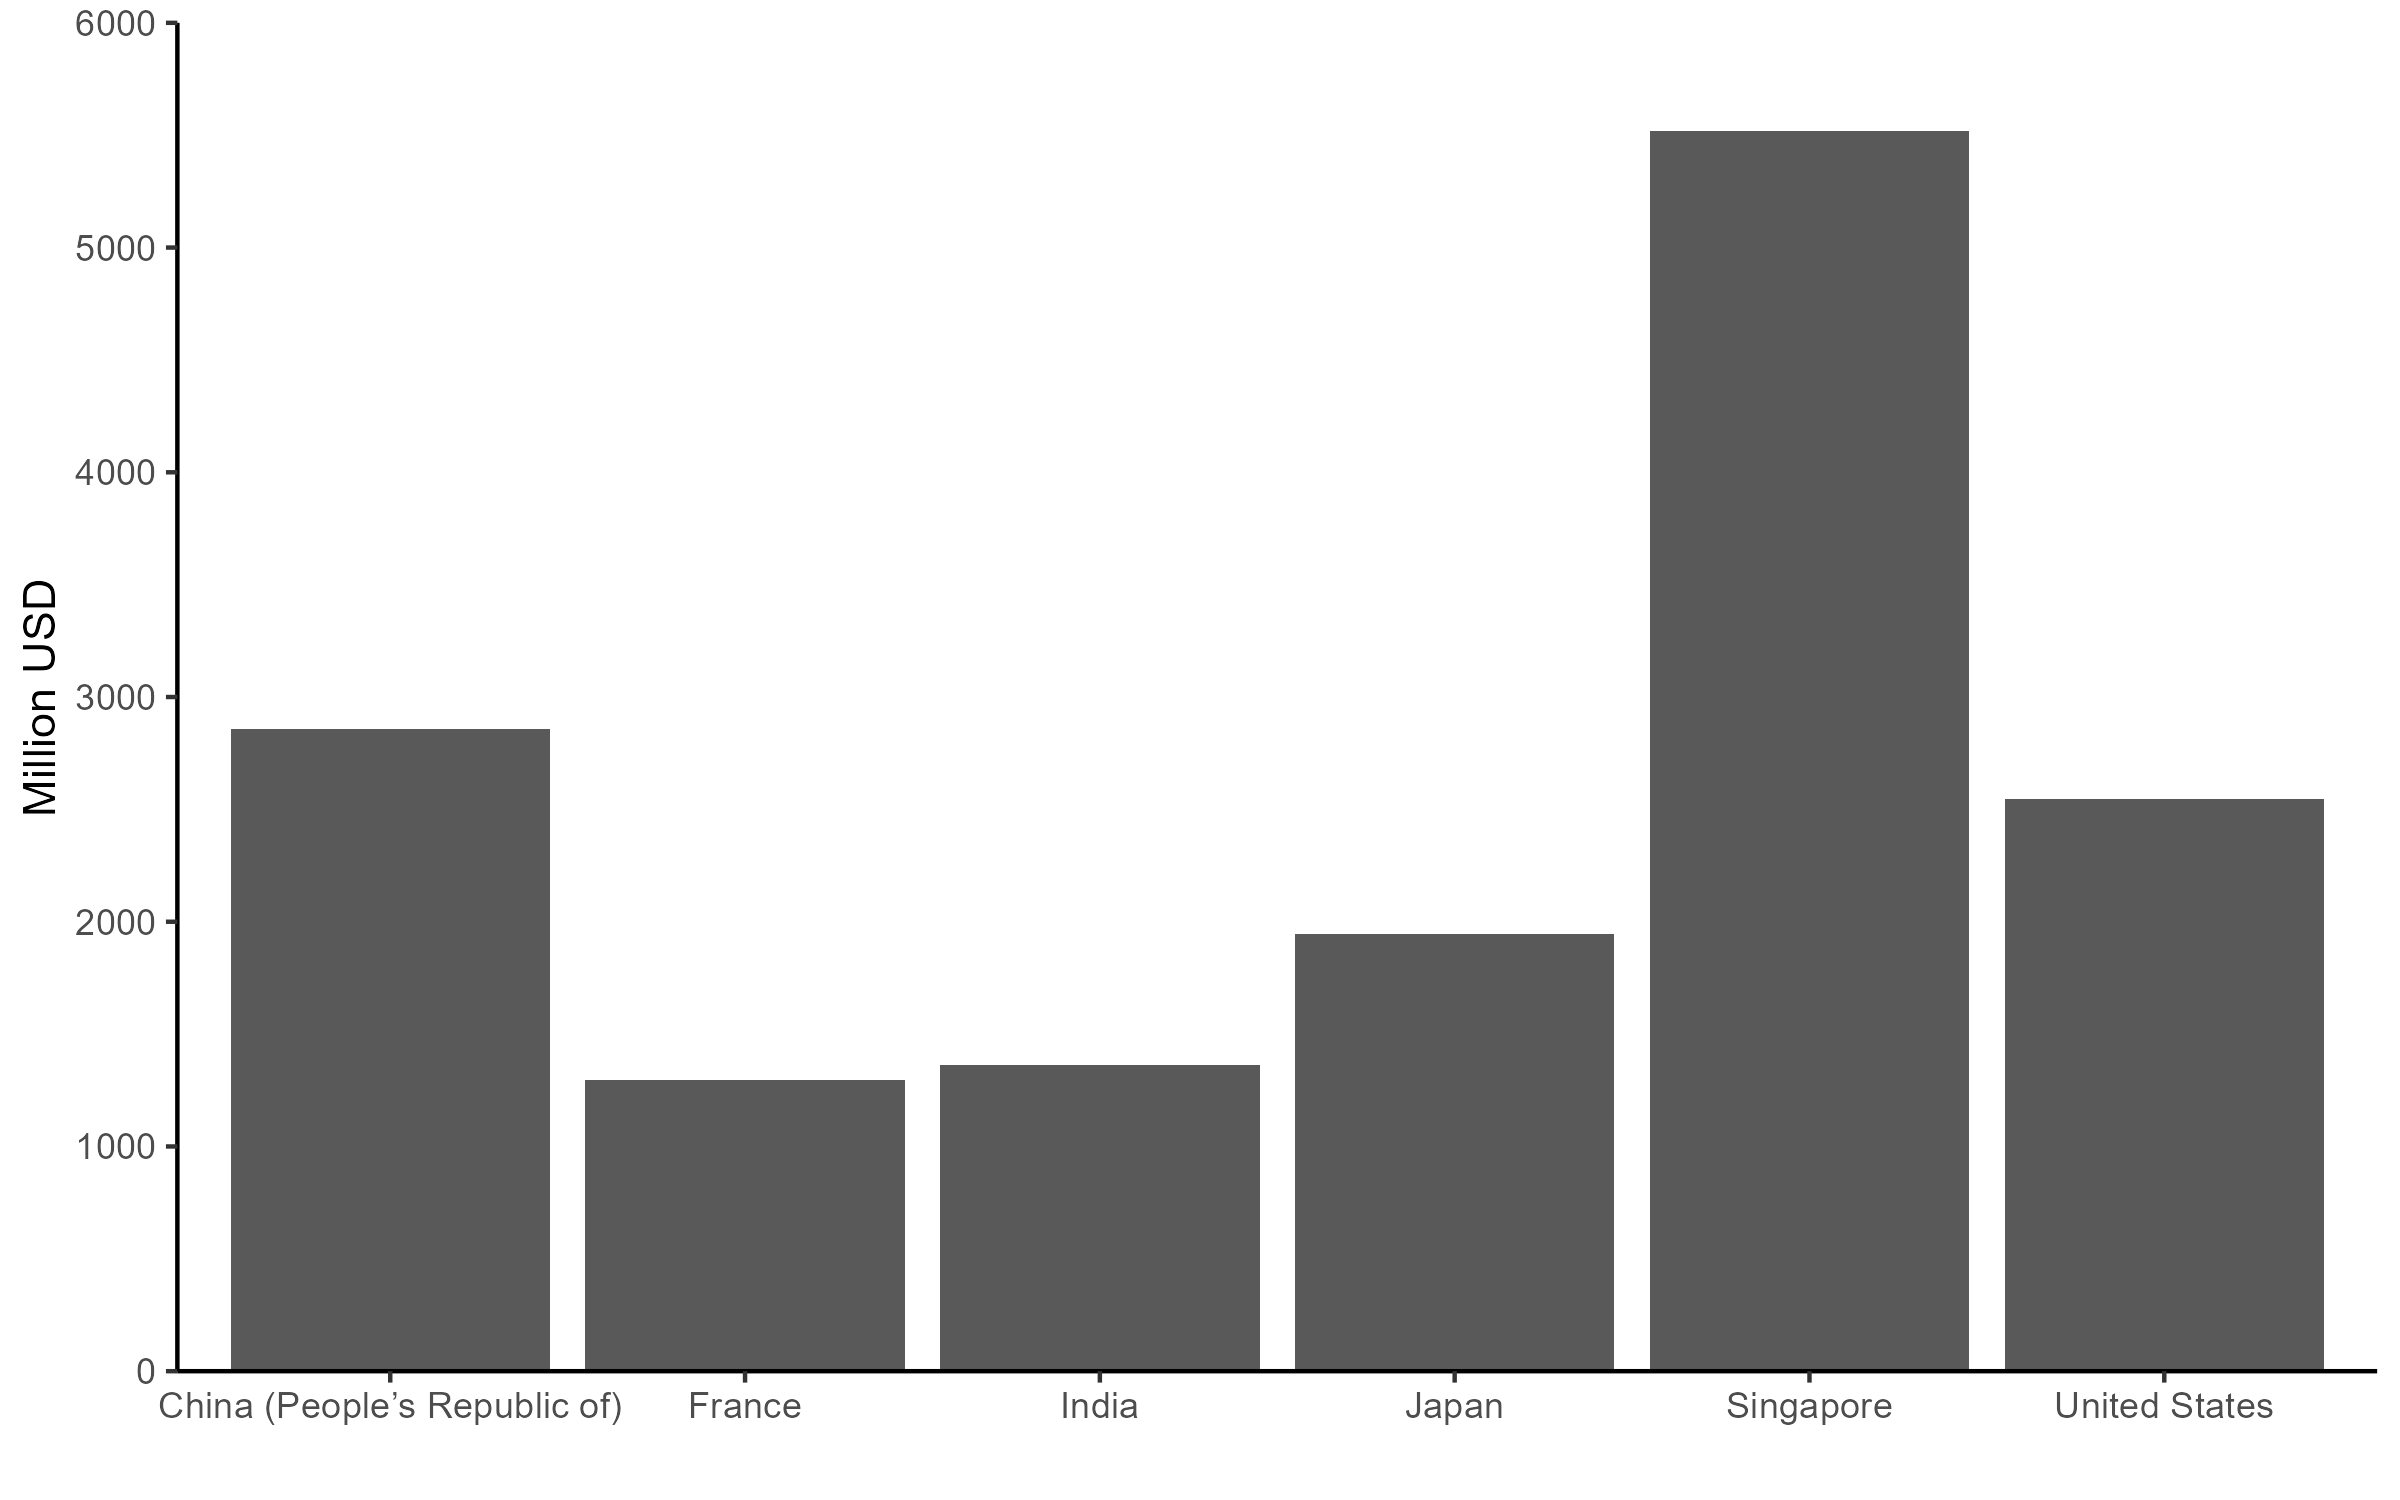
\includegraphics{plot/allcm.png}

}

\subcaption{\label{fig-CM}Indonesia's exports by partner, 2021}

\end{minipage}%
\newline
\begin{minipage}{0.50\linewidth}

\centering{

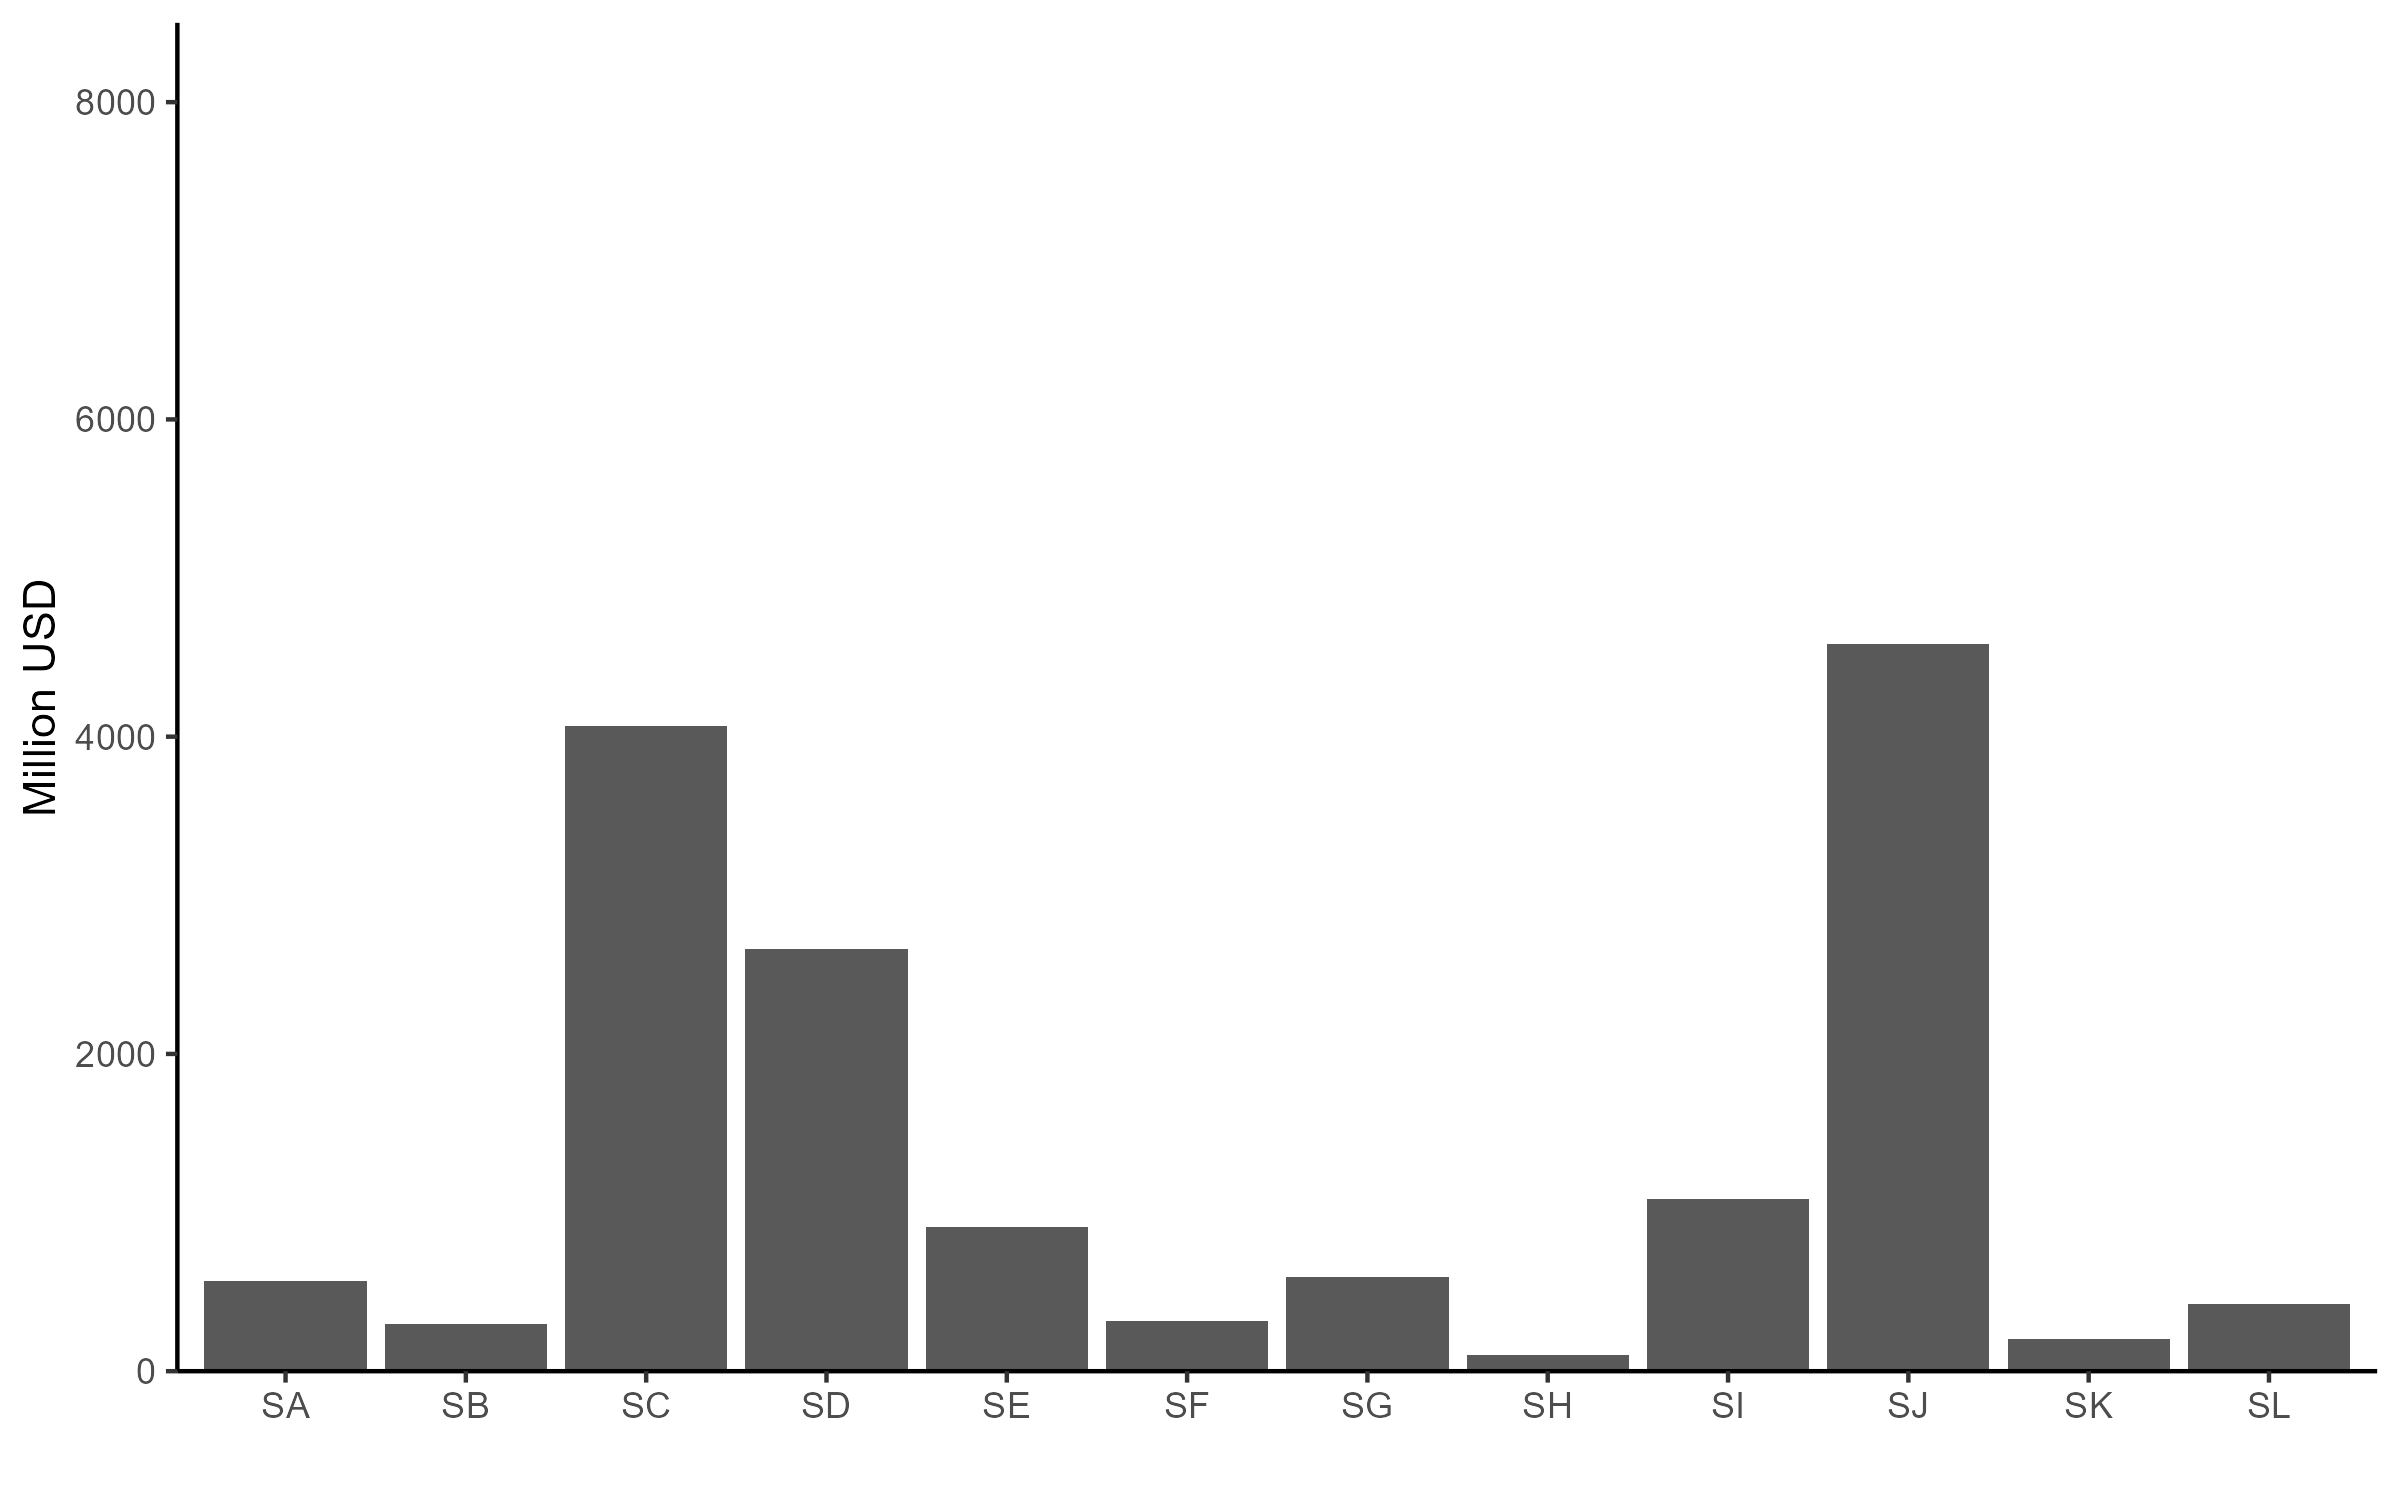
\includegraphics{plot/allsx.png}

}

\subcaption{\label{fig-SX}Indonesia's exports by sector, 2021}

\end{minipage}%
%
\begin{minipage}{0.50\linewidth}

\centering{

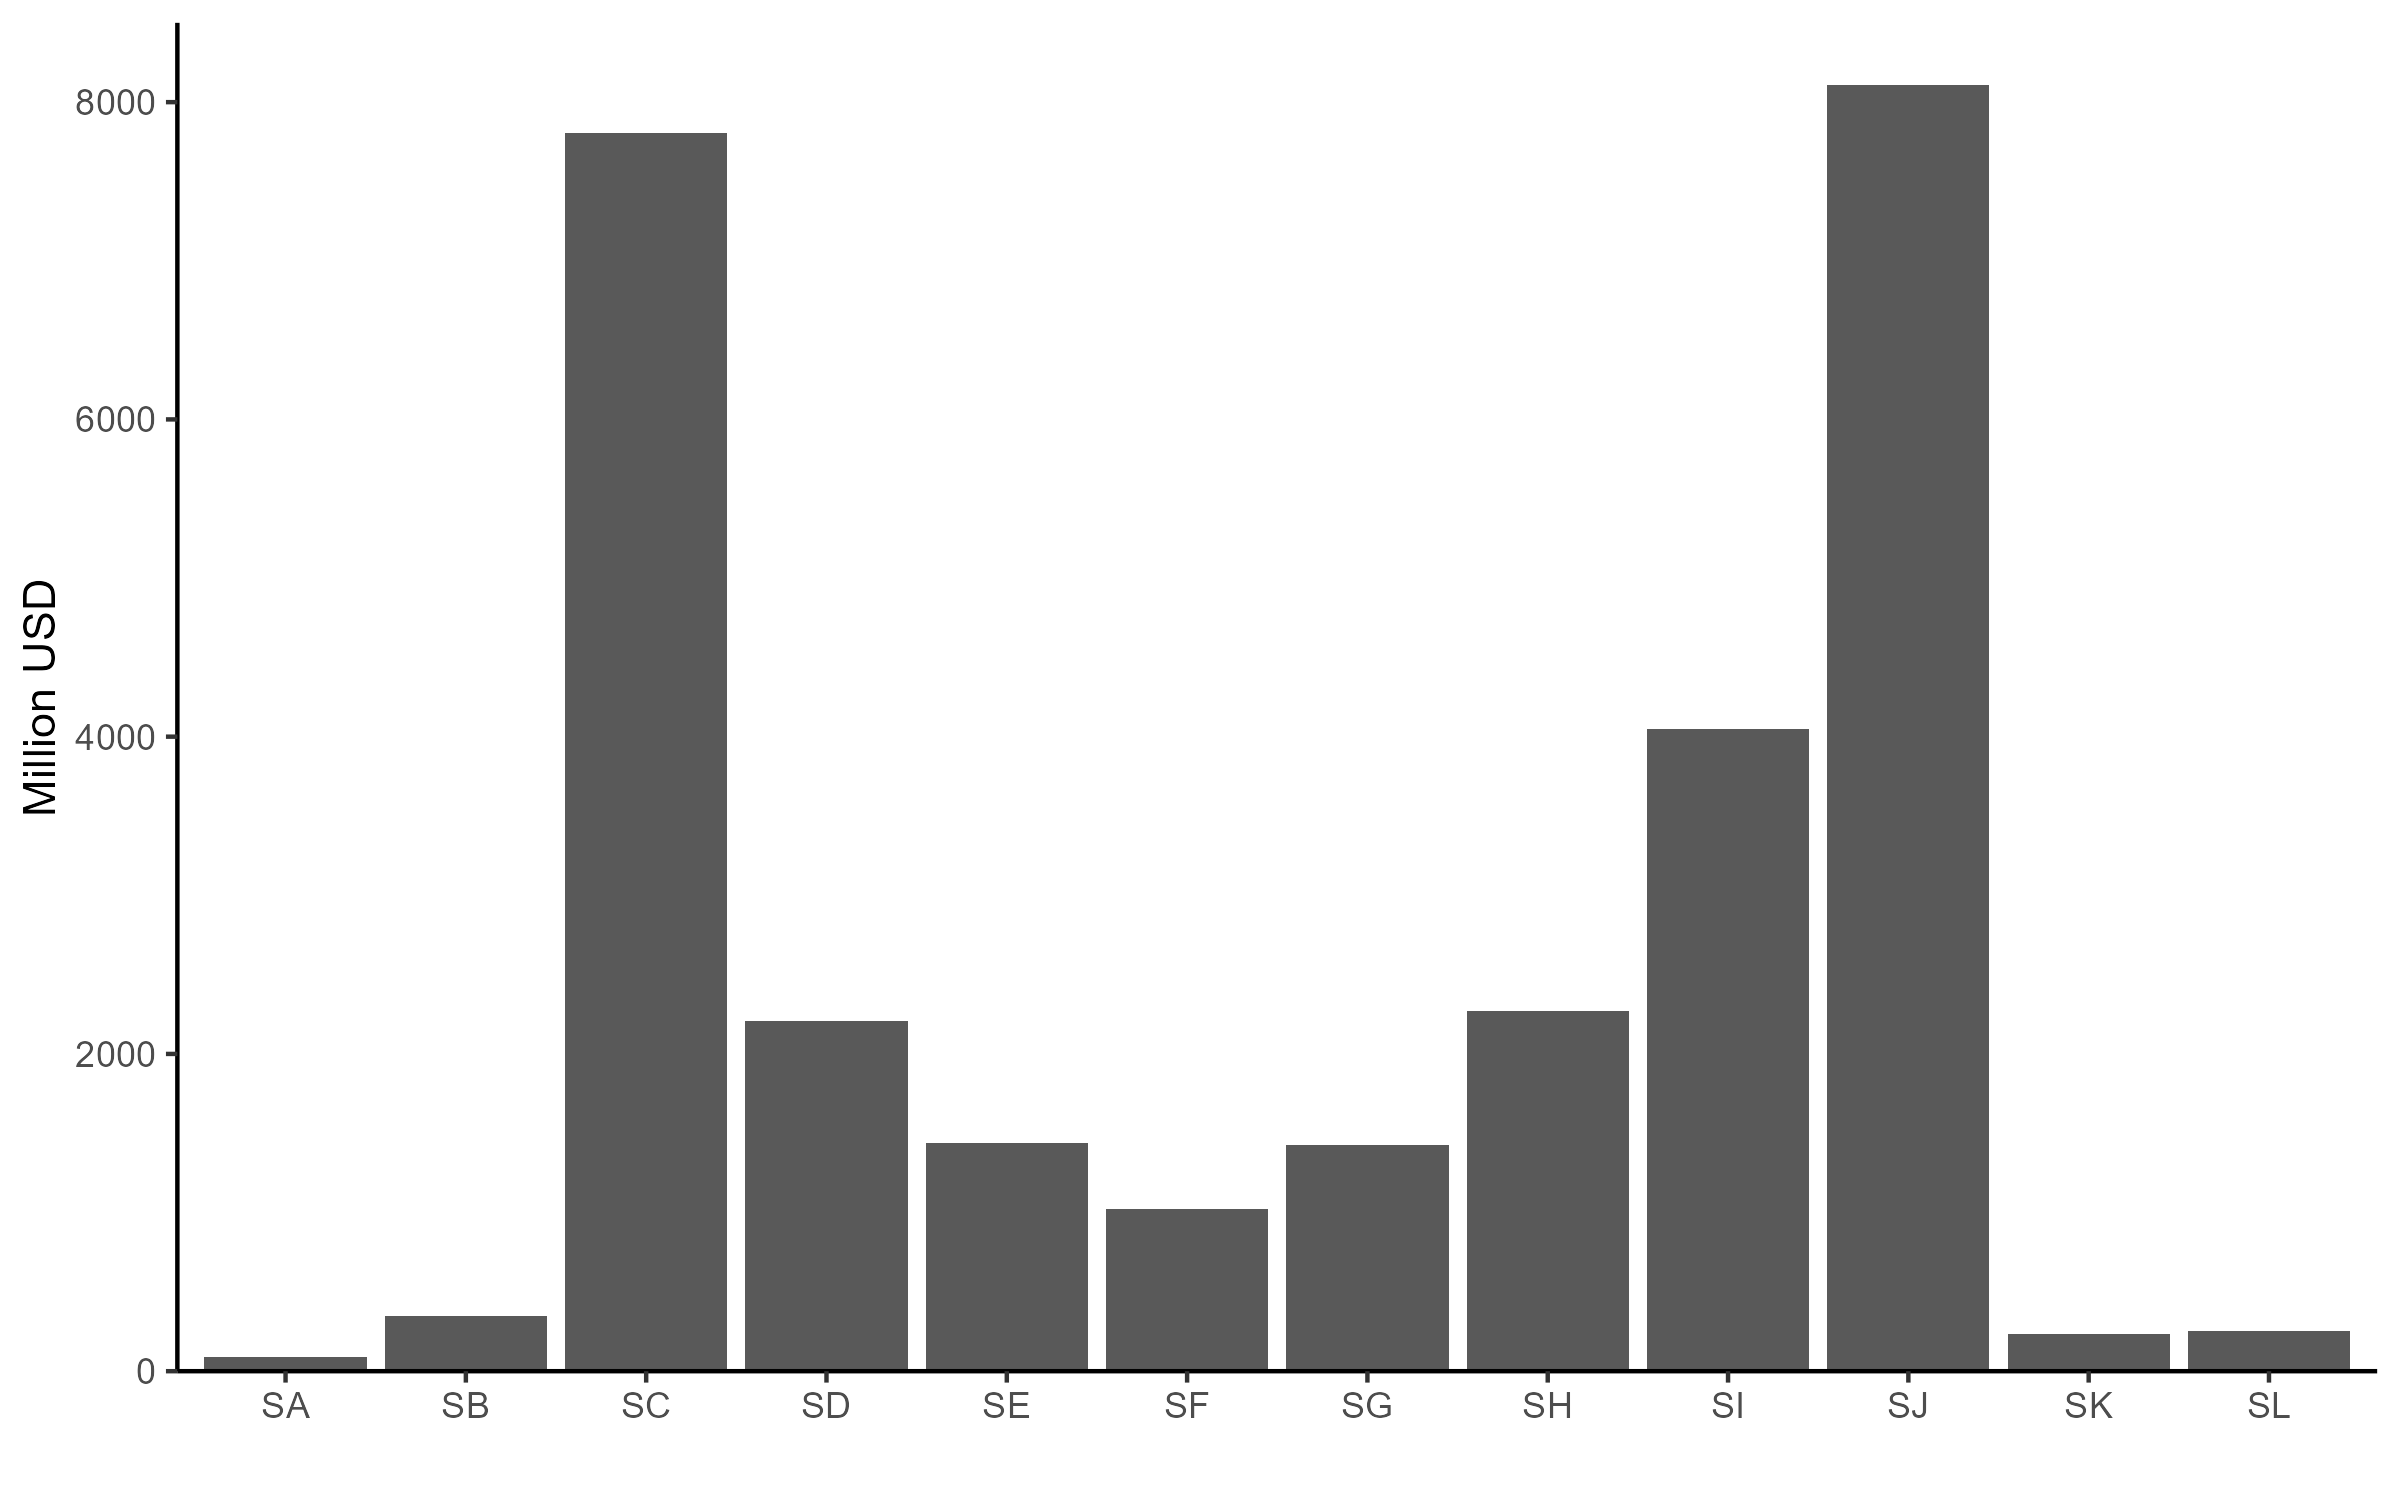
\includegraphics{plot/allsm.png}

}

\subcaption{\label{fig-SM}Indonesia's imports by sector, 2021}

\end{minipage}%

\caption{\label{fig-S}Indonesia's total services trade by categories,
2021}

\end{figure}%

We then focuses on Indonesia's four most important services. These are
transport (SC), travel (SD), ICT services (SI) and other business
services (SJ). Other business services includes consulting management,
research and development, and trade-related services (Liberatore et al.
2021). We look at top 6 partners in these sectors annually from
2005-2021 as existed in BaTIS, which can be seen in Figure~\ref{fig-X}
(exports) and Figure~\ref{fig-M} (imports). Some countries change
positions in these top 6 from time to time. A sudden miss of a country
does not mean it stops trading with Indonesia, it's just they got kicked
out of the top 6.

\begin{figure}

\begin{minipage}{0.50\linewidth}

\centering{

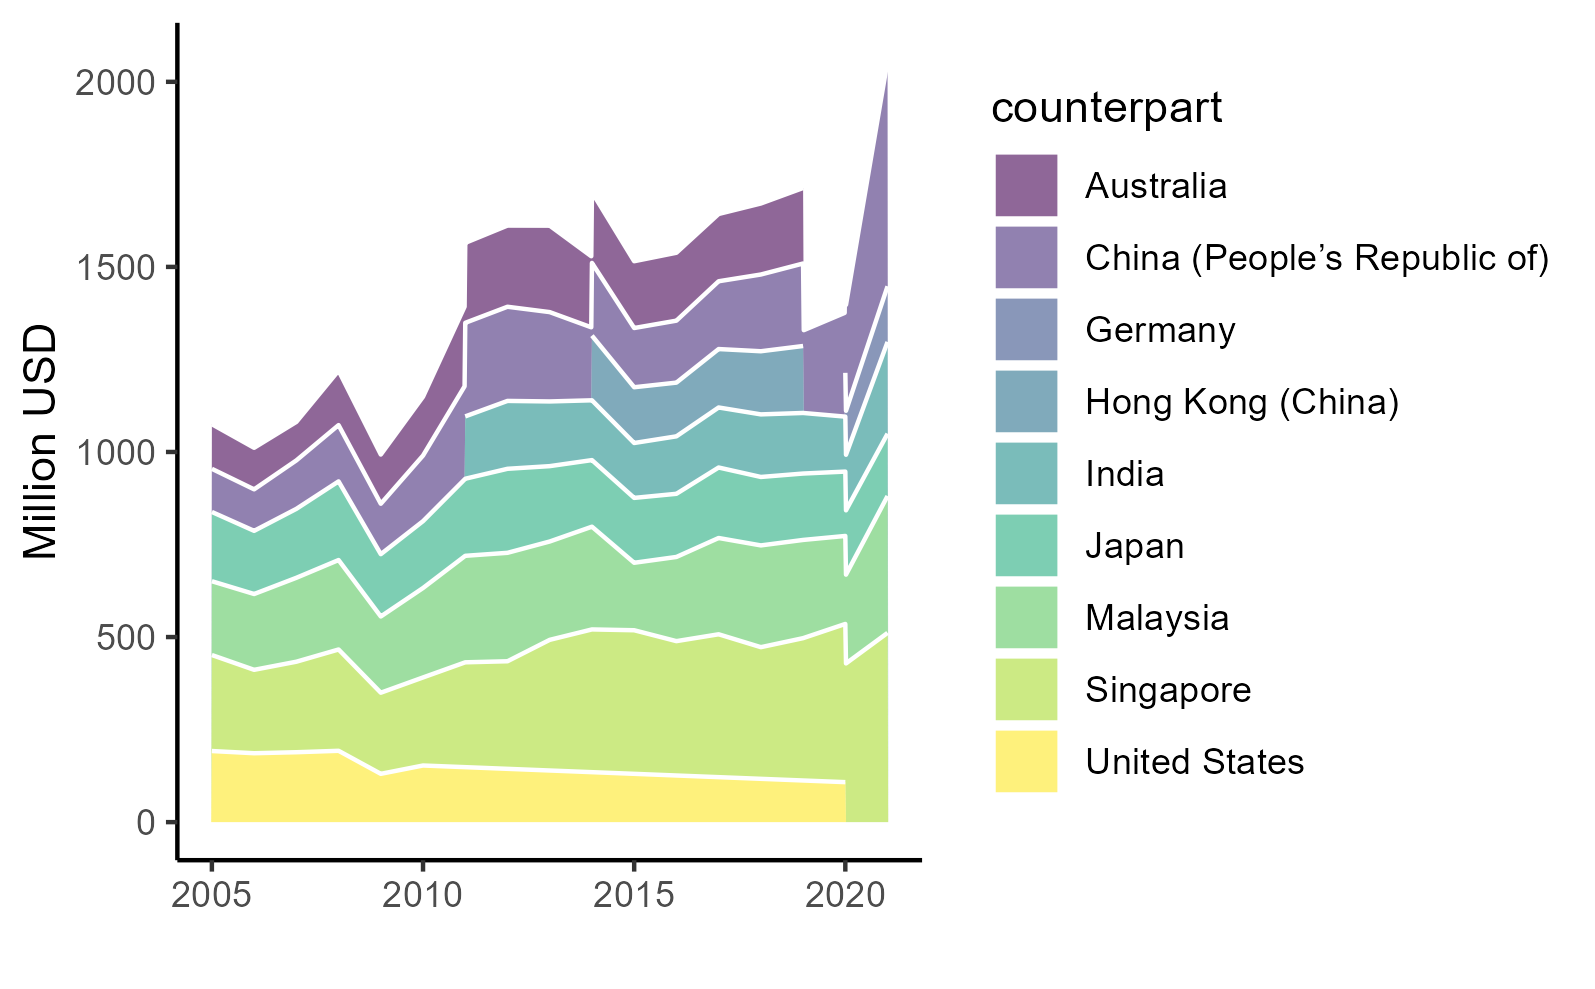
\includegraphics{plot/SCEX.png}

}

\subcaption{\label{fig-SCX}Transport}

\end{minipage}%
%
\begin{minipage}{0.50\linewidth}

\centering{

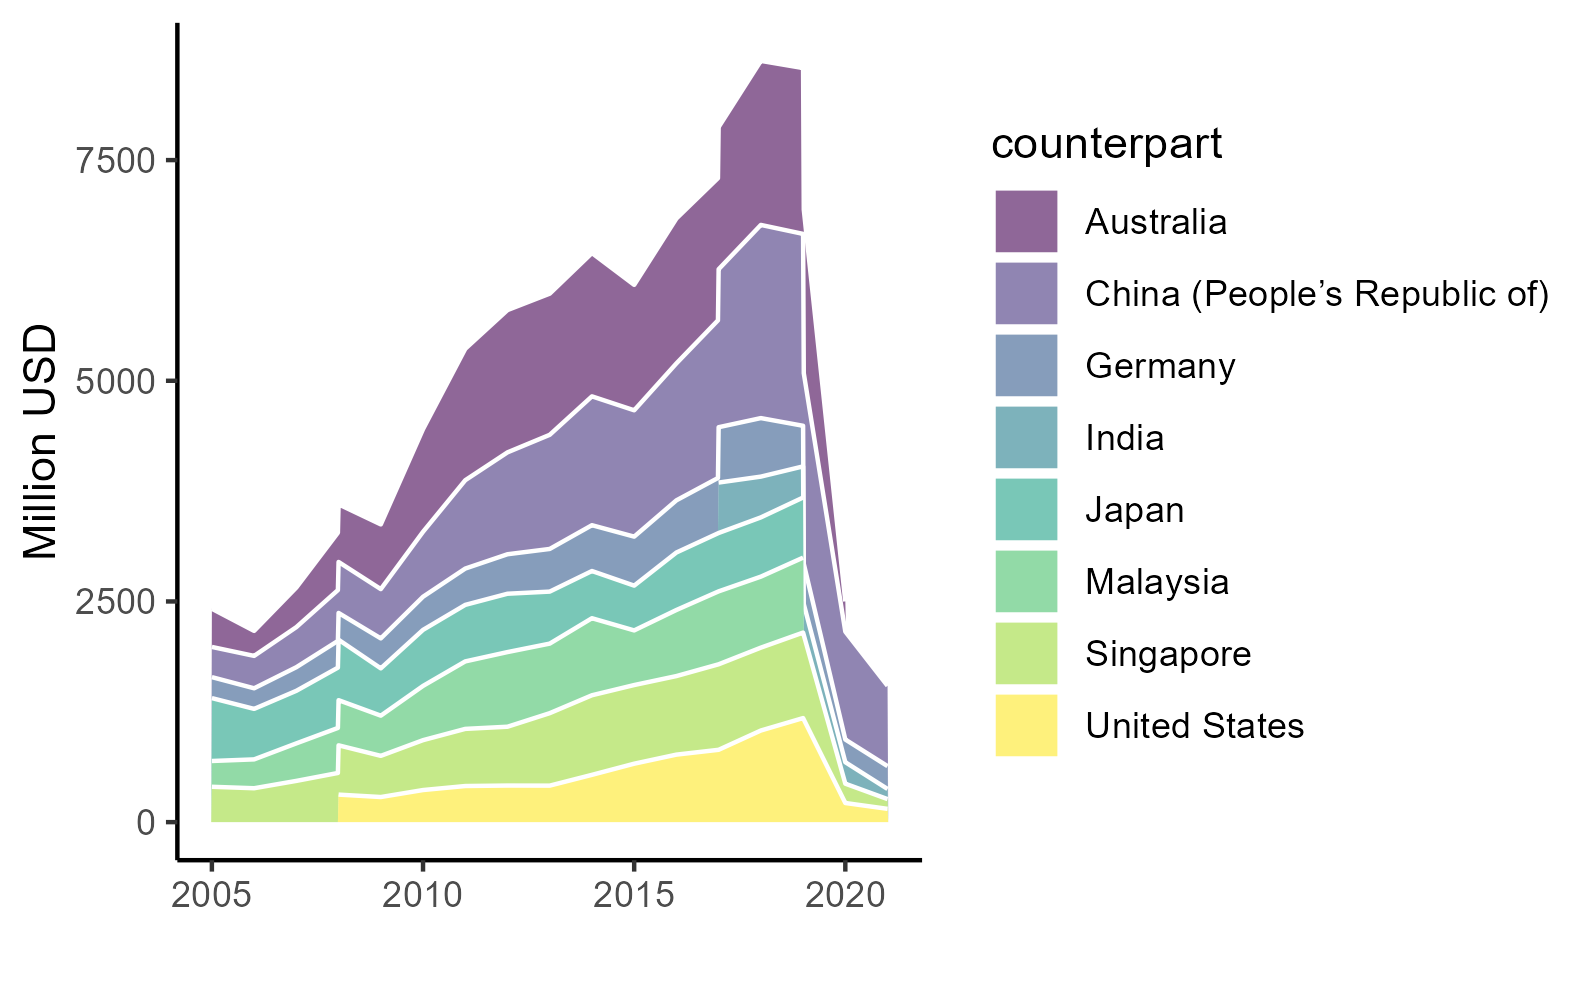
\includegraphics{plot/SDEX.png}

}

\subcaption{\label{fig-SDX}Travel}

\end{minipage}%
\newline
\begin{minipage}{0.50\linewidth}

\centering{

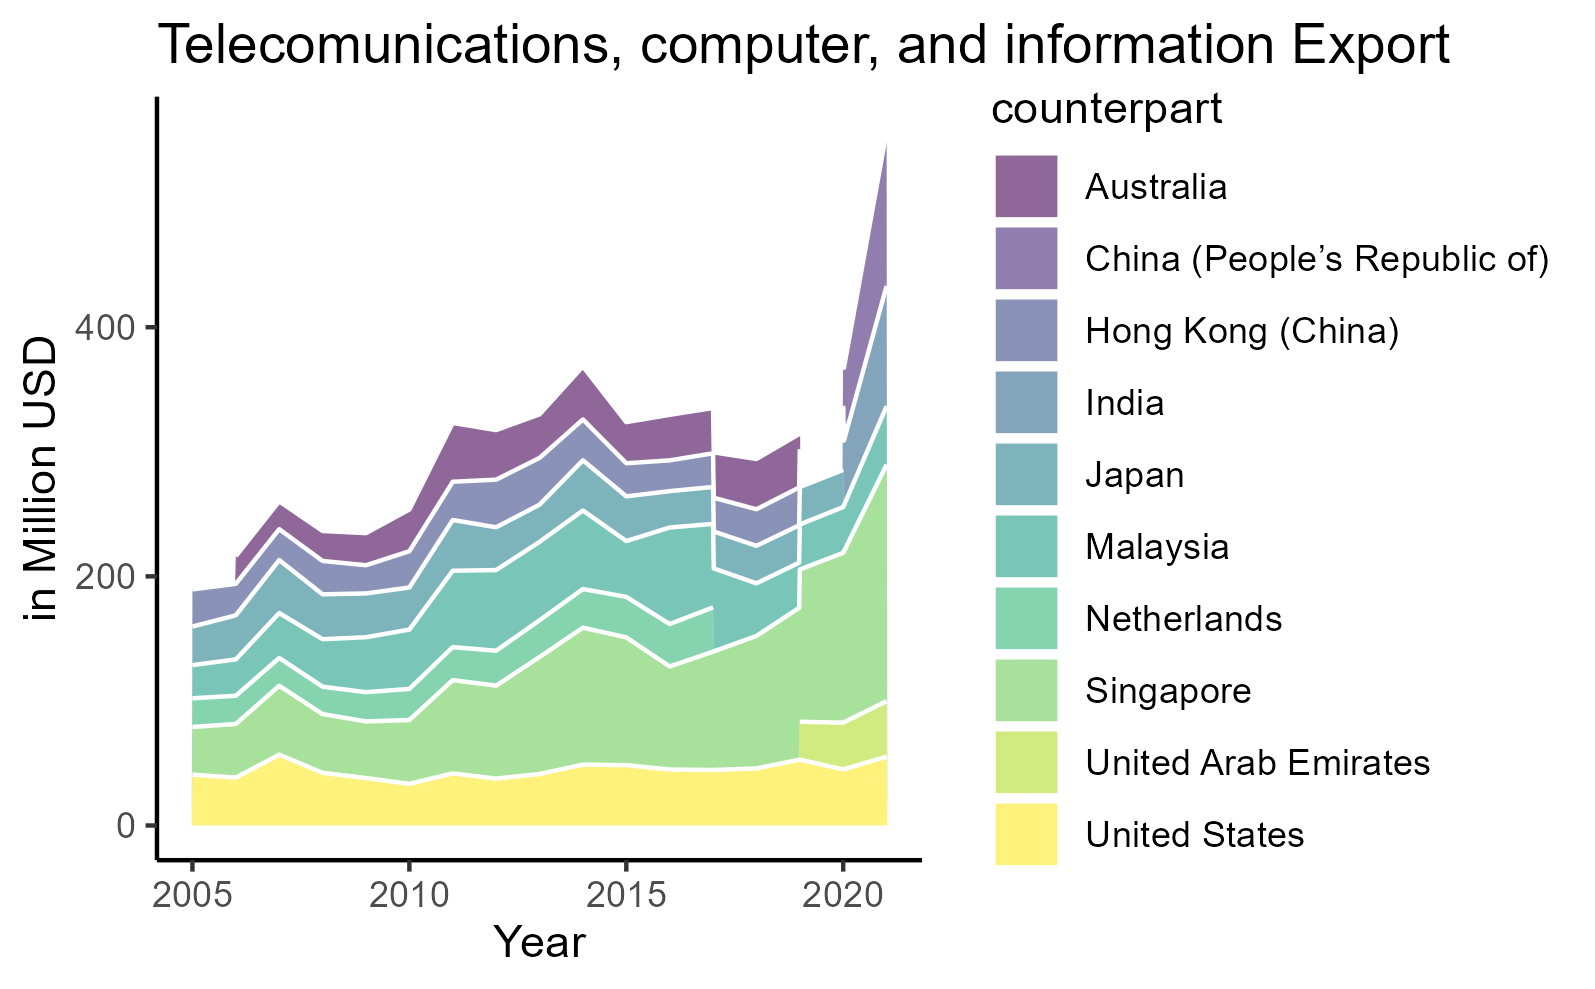
\includegraphics{plot/SIEX.png}

}

\subcaption{\label{fig-SIX}ICT services}

\end{minipage}%
%
\begin{minipage}{0.50\linewidth}

\centering{

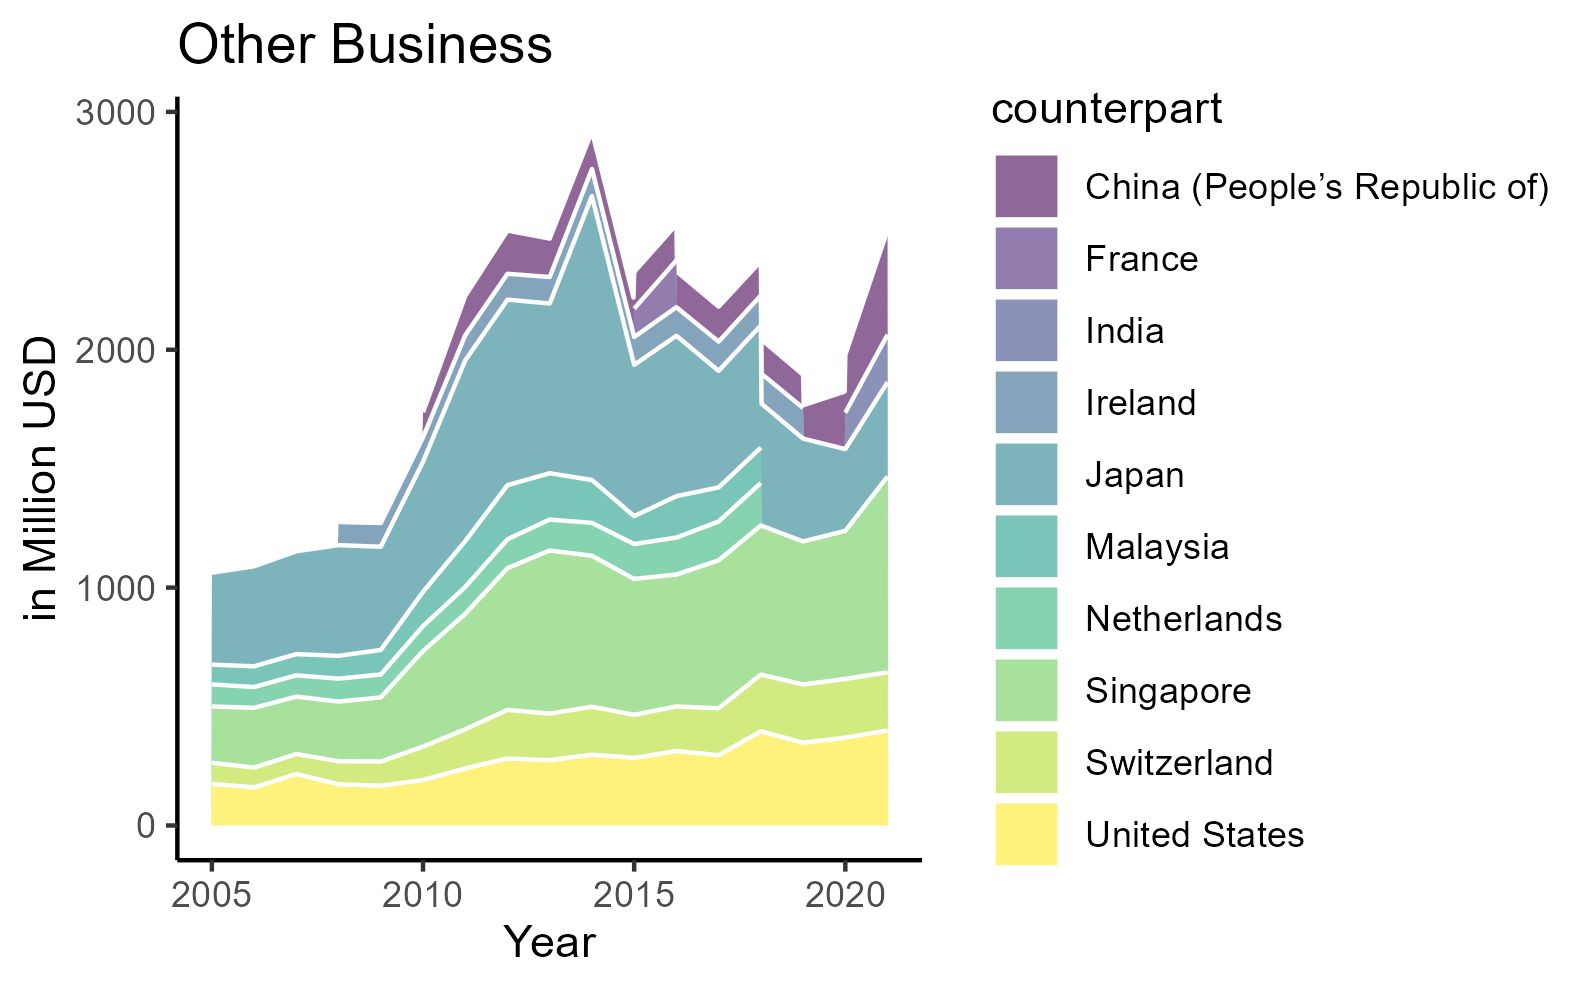
\includegraphics{plot/SJEX.png}

}

\subcaption{\label{fig-SJX}Other business services}

\end{minipage}%

\caption{\label{fig-X}Indonesia's top 6 exporters in 4 categories,
2005-2021}

\end{figure}%

\begin{figure}

\begin{minipage}{0.50\linewidth}

\centering{

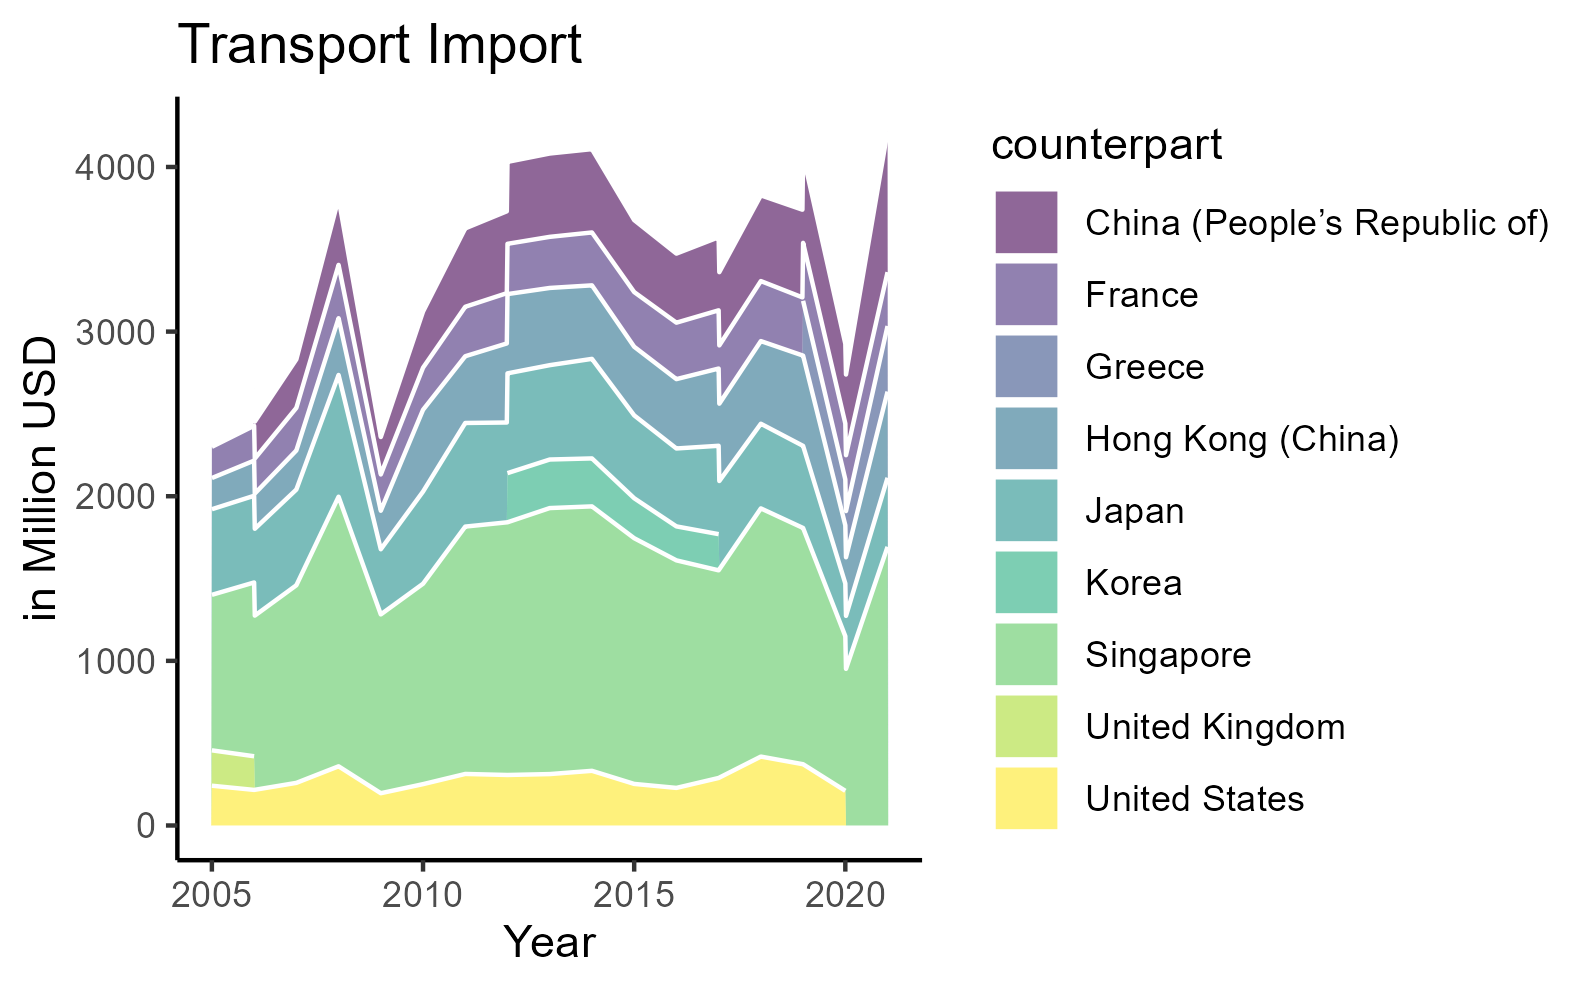
\includegraphics{plot/SCIM.png}

}

\subcaption{\label{fig-SCM}Transport}

\end{minipage}%
%
\begin{minipage}{0.50\linewidth}

\centering{

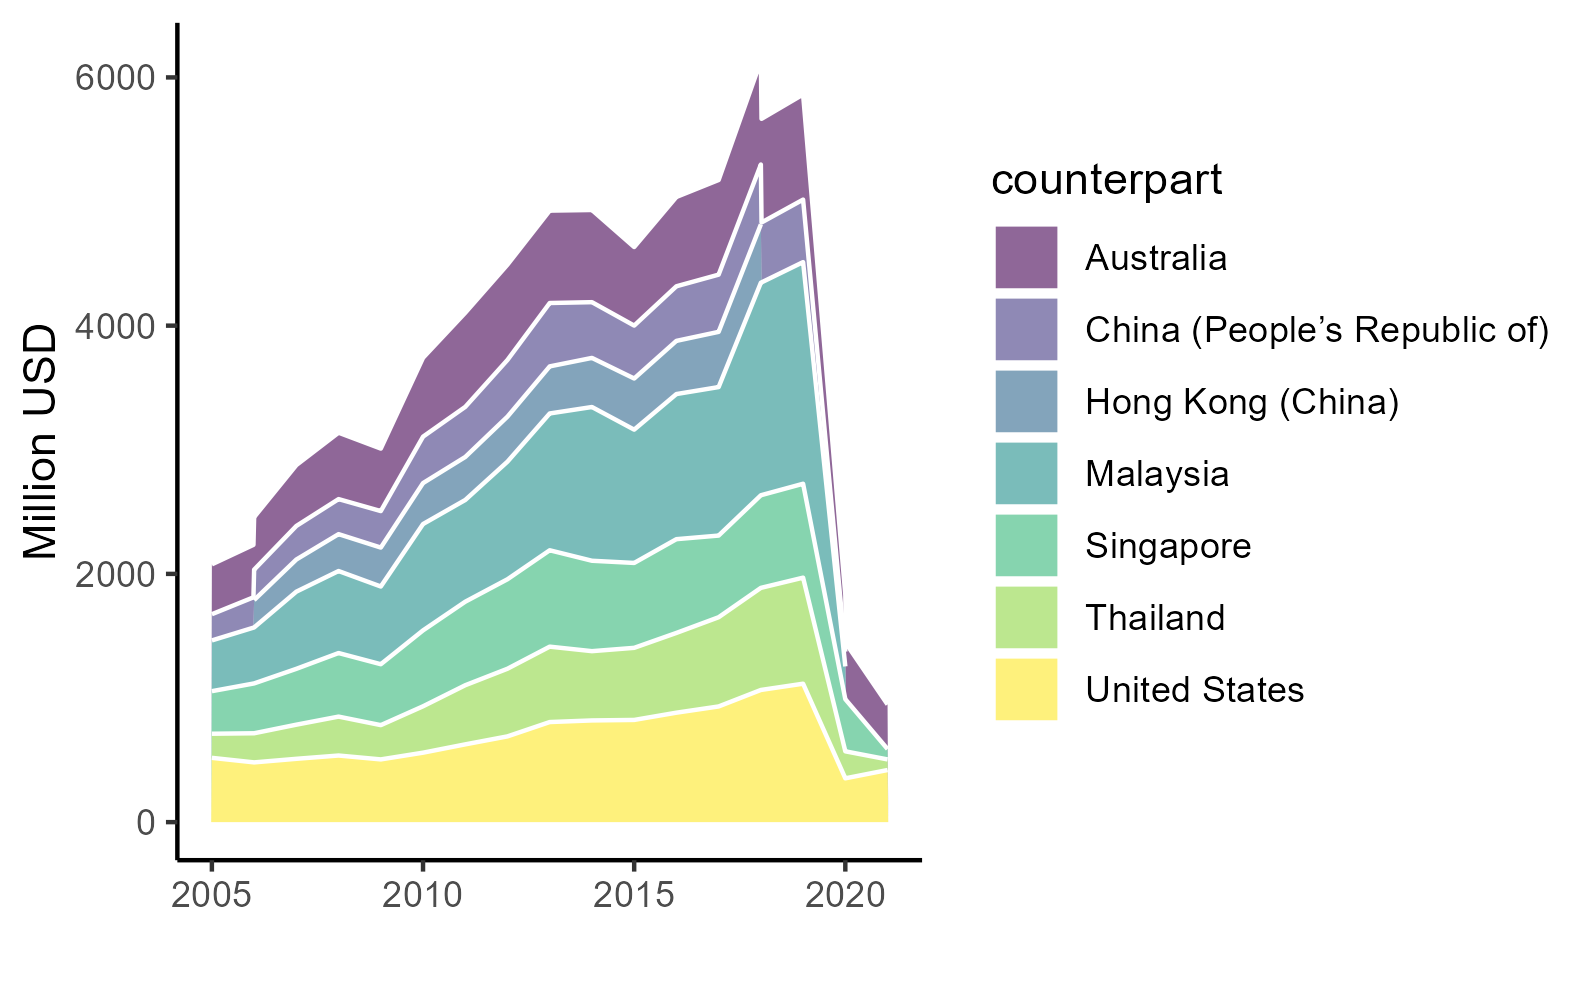
\includegraphics{plot/SDIM.png}

}

\subcaption{\label{fig-SDM}Travel}

\end{minipage}%
\newline
\begin{minipage}{0.50\linewidth}

\centering{

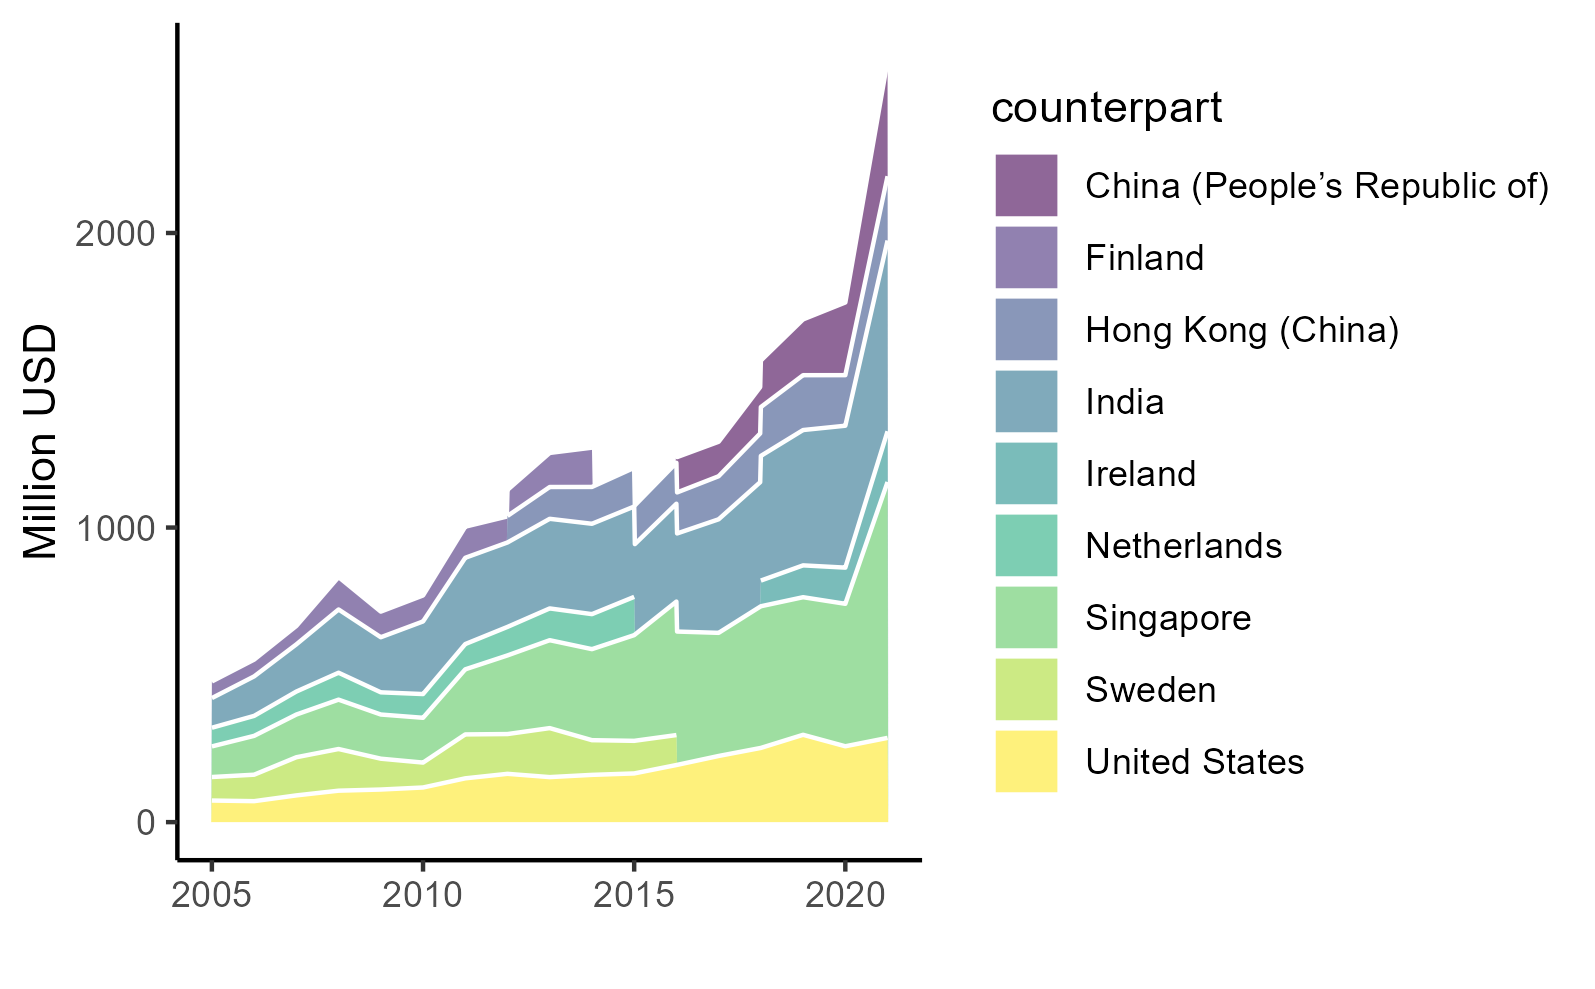
\includegraphics{plot/SIIM.png}

}

\subcaption{\label{fig-SIM}ICT services}

\end{minipage}%
%
\begin{minipage}{0.50\linewidth}

\centering{

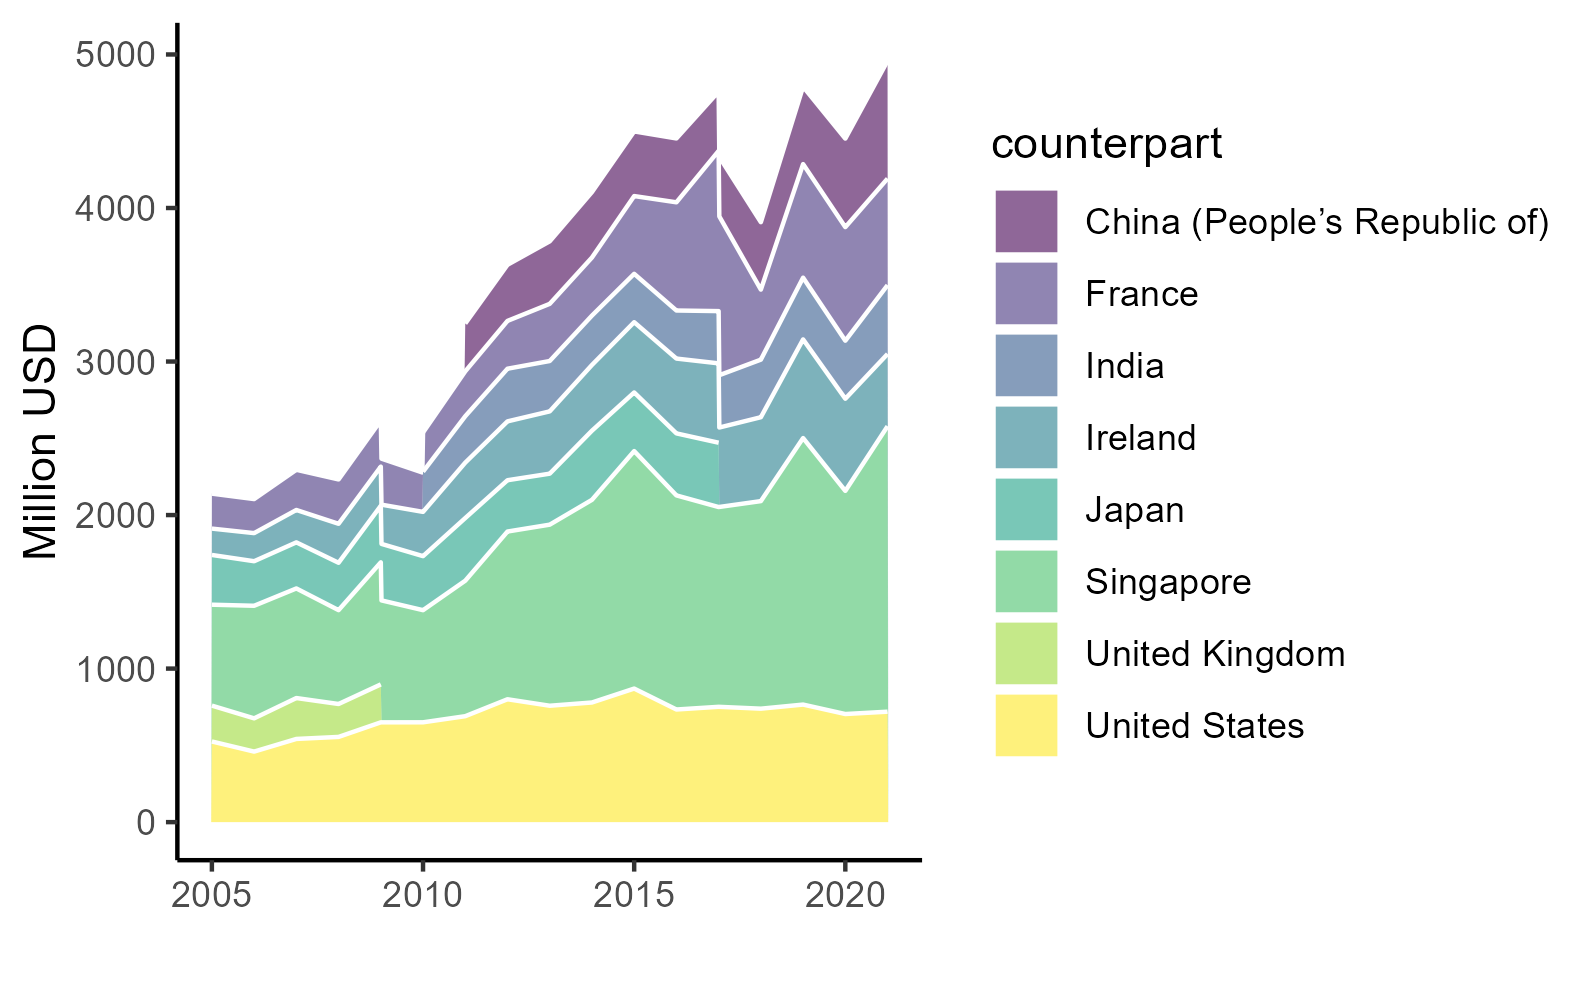
\includegraphics{plot/SJIM.png}

}

\subcaption{\label{fig-SJM}Other business services}

\end{minipage}%

\caption{\label{fig-M}Indonesia's top 6 importers in 4 categories,
2005-2021}

\end{figure}%

WHat we can immediately see is that there is a significant change
happened in 2020 and 2021, which corroborates the aggregated data in
Figure~\ref{fig-1}. This is likely due to the COVID-19 pandemic that
restrict movement of people.

This shock, however, affects differently between these four sectors. The
transportation sector decrease quite significantly in 2020, but
recovered back in 2021. The impact in the business services is milder
compared to the transportation sector. Meanwhile, we see a significant
drop in travel services and have not recovered since. Meanwhile, ICT
services are the winner here, with the top 6 partners experience
significant increase in both 2020 and 2021.

\subsection{Manufacturing}\label{manufacturing}

\subsubsection{General ARDL}\label{general-ardl}

\begin{figure}

\centering{

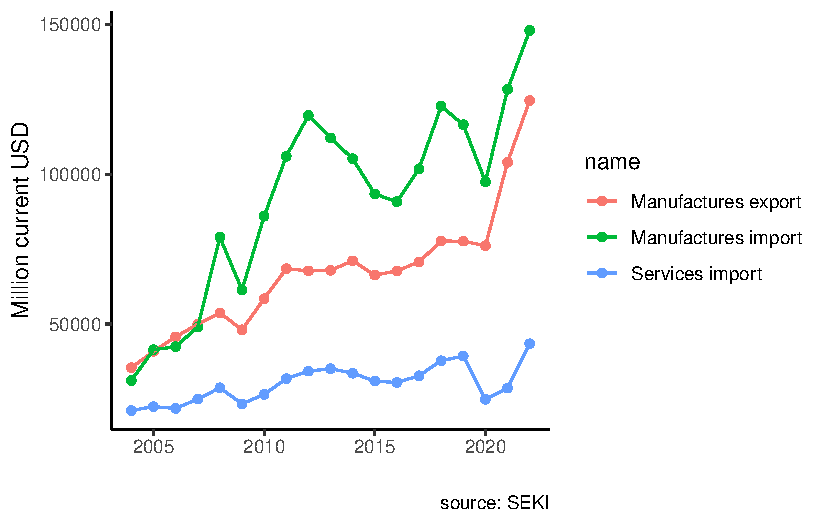
\includegraphics{services_document_files/figure-pdf/fig-idn-1.pdf}

}

\caption{\label{fig-idn}Indonesian trade dynamics}

\end{figure}%

\begin{table}

\caption{\label{tbl-2}ARDL results on four specifications}

\centering{

\centering
\begin{talltblr}[         %% tabularray outer open
entry=none,label=none,
note{}={+ p < 0.1, * p < 0.05, ** p < 0.01, *** p < 0.001},
]                     %% tabularray outer close
{                     %% tabularray inner open
colspec={Q[]Q[]Q[]Q[]Q[]},
column{1}={halign=l,},
column{2}={halign=c,},
column{3}={halign=c,},
column{4}={halign=c,},
column{5}={halign=c,},
hline{16}={1,2,3,4,5}{solid, 0.05em, black},
}                     %% tabularray inner close
\toprule
& Export 1 & Export 2 & GDP 1 & GDP 2 \\ \midrule %% TinyTableHeader
(Intercept) & \num{0.704}   & \num{1.354}+   & \num{0.112}    & \num{0.243}+   \\
& (\num{0.724}) & (\num{0.692})  & (\num{0.127})  & (\num{0.128})  \\
L(exM, 1)   & \num{0.676}** & \num{1.135}*** &                 &                 \\
& (\num{0.222}) & (\num{0.177})  &                 &                 \\
imM         & \num{0.273}   & \num{0.307}*   & \num{-0.003}   & \num{-0.023}   \\
& (\num{0.184}) & (\num{0.127})  & (\num{0.020})  & (\num{0.022})  \\
imSev       & \num{-0.106}  & \num{-0.130}   & \num{0.098}**  & \num{0.110}*** \\
& (\num{0.247}) & (\num{0.146})  & (\num{0.029})  & (\num{0.024})  \\
L(imM, 1)   &                & \num{-0.151}   &                 & \num{0.031}    \\
&                & (\num{0.166})  &                 & (\num{0.023})  \\
L(imSev, 1) &                & \num{-0.485}*  &                 & \num{-0.083}*  \\
&                & (\num{0.182})  &                 & (\num{0.030})  \\
L(pdb, 1)   &                &                 & \num{0.917}*** & \num{0.938}*** \\
&                &                 & (\num{0.024})  & (\num{0.022})  \\
Num.Obs.    & \num{18}      & \num{18}       & \num{18}       & \num{18}       \\
R2          & \num{0.881}   & \num{0.967}    & \num{0.997}    & \num{0.998}    \\
R2 Adj.     & \num{0.856}   & \num{0.953}    & \num{0.997}    & \num{0.998}    \\
AIC         & \num{-54.6}   & \num{-73.5}    & \num{-131.6}   & \num{-138.2}   \\
BIC         & \num{-50.1}   & \num{-67.3}    & \num{-127.2}   & \num{-131.9}   \\
Log.Lik.    & \num{32.291}  & \num{43.772}   & \num{70.818}   & \num{76.085}   \\
RMSE        & \num{0.04}    & \num{0.02}     & \num{0.00}     & \num{0.00}     \\
\bottomrule
\end{talltblr}

}

\end{table}%

\subsubsection{ICIO Panel data}\label{icio-panel-data}

\begin{figure}

\centering{

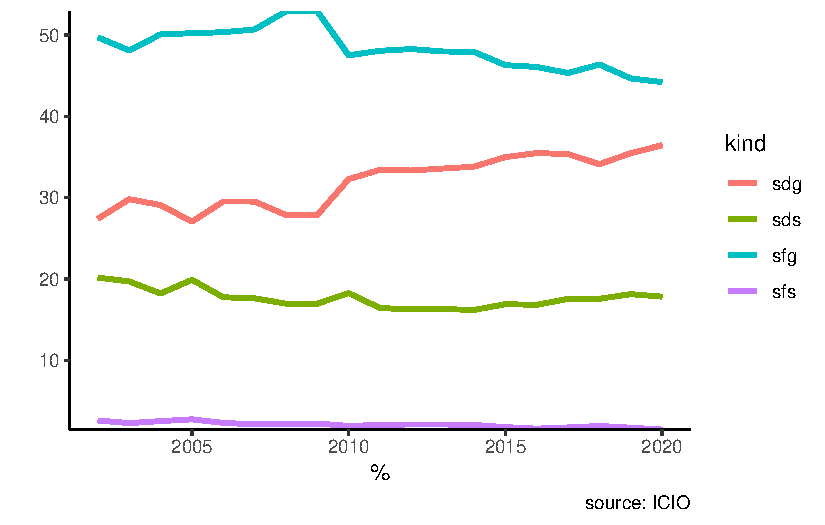
\includegraphics{services_document_files/figure-pdf/fig-indo-1.pdf}

}

\caption{\label{fig-indo}what}

\end{figure}%

\begin{table}

\caption{\label{tbl-sum2}Summary statistics}

\centering{

\centering
\begin{tblr}[         %% tabularray outer open
]                     %% tabularray outer close
{                     %% tabularray inner open
colspec={Q[]Q[]Q[]Q[]},
column{1}={halign=l,},
column{2}={halign=r,},
column{3}={halign=r,},
column{4}={halign=r,},
}                     %% tabularray inner close
\toprule
& Mean & Median & SD \\ \midrule %% TinyTableHeader
log value added             & \num{7.62} & \num{7.67} & \num{1.26} \\
log output                  & \num{9.01} & \num{9.06} & \num{1.21} \\
log foreign services share  & \num{5.98} & \num{6.00} & \num{1.21} \\
log domestic services share & \num{7.23} & \num{7.23} & \num{1.25} \\
\bottomrule
\end{tblr}

}

\end{table}%

\begin{table}

\caption{\label{tbl-regv}Panel regression of log manufacturing value
added}

\centering{

\centering
\begin{talltblr}[         %% tabularray outer open
entry=none,label=none,
note{}={+ p < 0.1, * p < 0.05, ** p < 0.01, *** p < 0.001},
]                     %% tabularray outer close
{                     %% tabularray inner open
colspec={Q[]Q[]Q[]Q[]Q[]Q[]Q[]},
column{1}={halign=l,},
column{2}={halign=c,},
column{3}={halign=c,},
column{4}={halign=c,},
column{5}={halign=c,},
column{6}={halign=c,},
column{7}={halign=c,},
hline{6}={1,2,3,4,5,6,7}{solid, 0.05em, black},
}                     %% tabularray inner close
\toprule
& all & IDN & SGP & VNM & THA & MYS \\ \midrule %% TinyTableHeader
lfs       & \num{0.159}    & \num{-0.207}  & \num{0.172}   & \num{0.358}**  & \num{-0.175}*  & \num{0.082}    \\
& (\num{0.159})  & (\num{0.283}) & (\num{0.170}) & (\num{0.094})  & (\num{0.062})  & (\num{0.264})  \\
lds       & \num{0.708}*** & \num{0.735}*  & \num{0.587}*  & \num{0.479}*** & \num{1.112}*** & \num{0.808}*** \\
& (\num{0.157})  & (\num{0.280}) & (\num{0.209}) & (\num{0.086})  & (\num{0.066})  & (\num{0.173})  \\
Num.Obs.  & \num{1520}     & \num{304}     & \num{304}     & \num{304}      & \num{304}      & \num{304}      \\
R2        & \num{0.825}    & \num{0.863}   & \num{0.984}   & \num{0.993}    & \num{0.992}    & \num{0.945}    \\
R2 Within & \num{0.658}    & \num{0.423}   & \num{0.780}   & \num{0.984}    & \num{0.952}    & \num{0.727}    \\
\bottomrule
\end{talltblr}

}

\end{table}%

We can see from Table~\ref{tbl-regv} that

\begin{table}

\caption{\label{tbl-rego}Panel regression of log manufacturing output}

\centering{

\centering
\begin{talltblr}[         %% tabularray outer open
entry=none,label=none,
note{}={+ p < 0.1, * p < 0.05, ** p < 0.01, *** p < 0.001},
]                     %% tabularray outer close
{                     %% tabularray inner open
colspec={Q[]Q[]Q[]Q[]Q[]Q[]Q[]},
column{1}={halign=l,},
column{2}={halign=c,},
column{3}={halign=c,},
column{4}={halign=c,},
column{5}={halign=c,},
column{6}={halign=c,},
column{7}={halign=c,},
hline{6}={1,2,3,4,5,6,7}{solid, 0.05em, black},
}                     %% tabularray inner close
\toprule
& all & IDN & SGP & VNM & THA & MYS \\ \midrule %% TinyTableHeader
lfs       & \num{0.221}+   & \num{-0.070}   & \num{0.179}   & \num{0.471}**  & \num{0.112}+   & \num{0.155}    \\
& (\num{0.105})  & (\num{0.141})  & (\num{0.138}) & (\num{0.135})  & (\num{0.062})  & (\num{0.166})  \\
lds       & \num{0.745}*** & \num{0.910}*** & \num{0.640}** & \num{0.547}*** & \num{0.865}*** & \num{0.745}*** \\
& (\num{0.103})  & (\num{0.129})  & (\num{0.166}) & (\num{0.123})  & (\num{0.062})  & (\num{0.103})  \\
Num.Obs.  & \num{1520}     & \num{304}      & \num{304}     & \num{304}      & \num{304}      & \num{304}      \\
R2        & \num{0.962}    & \num{0.954}    & \num{0.993}   & \num{0.995}    & \num{0.996}    & \num{0.987}    \\
R2 Within & \num{0.921}    & \num{0.880}    & \num{0.914}   & \num{0.990}    & \num{0.973}    & \num{0.891}    \\
\bottomrule
\end{talltblr}

}

\end{table}%

Meanwhile, we can see from Table~\ref{tbl-rego} the results from output
regression.

\section*{References}\label{references}
\addcontentsline{toc}{section}{References}

\phantomsection\label{refs}
\begin{CSLReferences}{1}{0}
\bibitem[\citeproctext]{ref-baldwin1}
Baldwin, Richard. 2011. {``21st Cebtury Regionalism: Filling the Gap
Between 21st Century Trade and 20th Century Trade Rules.''} Journal
Article. \emph{CEPR Policy Insight} 56.

\bibitem[\citeproctext]{ref-seki}
Bank Indonesia. n.d. {``Statistik Ekonomi Dan Keuangan Indonesia.''}
Dataset. Bank Indonesia,.
\url{https://www.bi.go.id/id/statistik/ekonomi-keuangan/seki/Default.aspx\#headingFour}.

\bibitem[\citeproctext]{ref-kimura1}
Kimura, Fukunari. 2018. {``Unbundling Regimes and Development Strategies
in ASEAN: Old Issues and New Challenges.''} Journal Article.
\emph{Southeast Asian Economies} 35 (1): 13--21.
\url{https://doi.org/10.1355/ae35-1c}.

\bibitem[\citeproctext]{ref-ebops}
Liberatore, Antonella, Rodolfo Ostolaza, Malik Bani Hani, Silvia Amiel,
Maria Fernanda L'Hopital, Markie Muryawan, Vysaul Nyirongo, and Habibur
Khan. 2021. {``C.6 Trade in Services Classifications.''} Report.
International Monetary Fund.
\url{https://www.imf.org/external/pubs/ft/bop/2021/pdf/VM2/21-05.pdf}.

\bibitem[\citeproctext]{ref-batis2}
Liberatore, Antonella, and Steen Wettstein. 2021. {``The OECD-WTO
Balanced Trade in Services Database (BaTIS).''} Report. OECD/WTO.
\url{https://www.oecd.org/content/dam/oecd/en/data/methods/OECD-WTO-Balanced-Trade-in-Services-database-methodology-BPM6.pdf}.

\bibitem[\citeproctext]{ref-ardl}
Natsiopoulos, Kleanthis, and TNickolaos G Tzeremes. 2022. {``ARDL Bounds
Test for Countegration: Replicating the Pesaran Et Al. (2001) Results
for the UK Earnings Equation Using r.''} Journal Article. \emph{Journal
of Applied Econometrics} 37 (5): 22.
\url{https://doi.org/doi.org/10.1002/jae.2919}.

\bibitem[\citeproctext]{ref-icio}
OECD. 2023. {``OECD Inter-Country Input-Output Database.''} Dataset.
\url{http://oe.cd/icio}.

\bibitem[\citeproctext]{ref-aco}
Patunru, Arianto A. 2023. {``Trade Policy in Indonesia: Between
Ambivalence, Pragmatism and Nationalism.''} Journal Article.
\emph{Bulletin of Indonesian Economic Studies} 59 (3): 311--40.
\url{https://doi.org/10.1080/00074918.2023.2282821}.

\bibitem[\citeproctext]{ref-pesaran}
Pesaran, M. Hashem, and Ron Smith. 1995. {``Estimating Long-Run
Relationships from Dynamic Heterogeneous Panels.''} Journal Article.
\emph{Journal of Econometrics} 68 (1): 79--113.
https://doi.org/\url{https://doi.org/10.1016/0304-4076(94)01644-F}.

\bibitem[\citeproctext]{ref-batis1}
WTO/OECD. 2022. {``OECD-WTO: Balanced International Trade in Services -
EBOPS 2002 (Edition 2021).''} Dataset. OECD Statistics on International
Trade in Services (database). \url{https://doi.org/10.1787/54a469fc-en}.

\end{CSLReferences}



\end{document}
